\chapter{Fluctuation de la distribution de rapidité dans des état d'équilibre}
\label{chap:Fluctu} 
\minitoc

\section*{Introduction}

\paragraph{Pourquoi étudier les fluctuations ?}

L’hypothèse selon laquelle, après relaxation, le système est décrit par un \textit{Generalized Gibbs Ensemble} (GGE) constitue un fondement majeur de notre compréhension des dynamiques hors équilibre dans les systèmes intégrables. Cette hypothèse, bien que robuste théoriquement, appelle à être testée expérimentalement.

Toutefois, la seule connaissance de la distribution de rapidité moyenne \( \rho_{\mathrm{eq}} \) ne permet pas, à elle seule, de confirmer la validité du GGE. En effet, plusieurs ensembles statistiques peuvent mener à une même valeur moyenne de \( \rho(\theta) \). Pour lever cette ambiguïté, il est nécessaire d’étudier les \textbf{fluctuations} autour de la distribution typique, notées \( \delta \rho \), définies par :
\(
\rho = \rho_{\mathrm{eq}} + \delta \rho.
\)
Cela nécessite de pousser le développement fonctionnel de la \emph{fonction thermodynamique effective} \( (\mathcal{S}_{YY} - \mathcal{W})[\rho] \) à l’ordre quadratique en \( \delta \rho \).

\medskip
Si la GGE décrit correctement la valeur moyenne de \( \rho(\theta) \) après relaxation, il est naturel de se demander si elle capture également les \emph{fluctuations} autour de cette moyenne. Autrement dit, notre objectif est de tester si la GGE constitue le \textit{bon ensemble statistique} pour l’état stationnaire, en analysant non seulement la distribution moyenne des quasi-particules, mais aussi ses fluctuations.\\

{\color{blue} { \color{red} (en traveaux , ... les articles sont a lire plus en détails mais voilas un début)} 
\medskip
Plusieurs travaux récents ont mis en lumière l’intérêt expérimental de sonder ces fluctuations. De Nardis et al.\ ont notamment montré que la mesure de la \textit{structure dynamique} de la densité, après un quench, permet de reconstruire entièrement l’état stationnaire, c’est-à-dire la distribution \( \rho(\theta) \) du GGE~\cite{DeNardis2017}. En particulier, l’analyse du facteur de structure dynamique permet d’extraire les différentes \textit{températures effectives} \( \beta_i \) du GGE, et donc d’accéder à la distribution macroscopique des quasi-particules~\cite{Goldstein2013,CauxKonik2012}.

\medskip
Ainsi, en mesurant les corrélations dynamiques du gaz — accessibles expérimentalement via la spectroscopie ou les fluctuations de densité — on peut tester si les fluctuations observées concordent avec celles prédites par la GGE.

\medskip
Concrètement, cela consiste à analyser la dispersion des vitesses (ou rapidités) sur plusieurs répétitions expérimentales d’un même quench. Si la GGE décrit correctement l’état stationnaire, la variance et les corrélations des fluctuations de \( \rho(\theta) \) devraient être en accord avec les prédictions du formalisme fluctuationnel issu de l’entropie \( \operator{\rho}^{(\mathcal{S})}_{\mathrm{GGE}} \), cf.~\eqref{chap.TBA.op.rho.S}.

\medskip
Le lien entre fluctuations, fonctions de réponse, et ensembles de Gibbs généralisés (GGE) a suscité un intérêt croissant dans les systèmes quantiques intégrables. Le formalisme des charges quasi-locales et des potentiels conjugués dans le GGE a été précisé dans le modèle de Lieb–Liniger par Pálmai et Konik~\cite{Palmai2018}, qui montrent comment structurer la matrice densité en termes de fonctionnelles de rapidité. L'identité fondamentale liant la dérivée fonctionnelle de l'entropie de Yang–Yang au noyau de fluctuations $\chi(\theta,\theta')$ est également dérivée dans ce cadre.

La relation fluctuation–réponse dans les gaz bosoniques unidimensionnels a été étudiée en profondeur par De Nardis et al.~\cite{DeNardis2017}, qui proposent une méthode pour reconstruire les fluctuations thermiques à partir de fonctions de réponse dynamiques, en comparant mesures expérimentales et théories thermodynamiques. D'autres travaux, comme ceux de Goldstein et Andrei~\cite{Goldstein2013}, ou de Caux et Konik~\cite{CauxKonik2012}, examinent en détail la relaxation vers un GGE à la suite d’un quench quantique, et en particulier le rôle de la distribution de rapidité dans la description des états stationnaires.

%Enfin, les travaux de Essler, Mussardo et Panfil~\cite{Essler2015} donnent une perspective unificatrice dans le cadre des théories de champs intégrables, où la fluctuation–réponse s’exprime à partir de noyaux intégrables et de corrélateurs généralisés.
}

\medskip
En résumé, l’étude des fluctuations de la distribution de rapidités fournit un test clé de la validité du GGE pour modéliser les résultats expérimentaux dans le modèle de Lieb–Liniger~\cite{DeNardis2017}.

\medskip
Ce chapitre est consacré à cette extension, qui permettra :
\begin{itemize}[label = $\bullet$]
  \item d’obtenir les matrices de susceptibilité \(\chi_{w}\)  et les corrélations gaussiennes du GGE ;
  %\item de relier ces fluctuations aux observables expérimentales  (temps de vol, bruit de densité, etc.) ;
  \item de fournir la base théorique des équations d’hydrodynamique généralisée au second ordre.
\end{itemize}

Nous commencerons par rappeler le formalisme variationnel, puis nous dériverons l’action quadratique régissant \(\delta\rho\).  %Les contraintes d’intégrabilité et la structure du noyau \(\Delta\) joueront un rôle clé dans la diagonalisation de cette action, ouvrant la voie aux prédictions quantitatives sur les fluctuations GGE.


\section{Fluctuation-réponse et susceptibilités dans les états d’équilibre généralisés}

Soient $\omega$, $f$ et $g$ des fonctions.

La dérivée fonctionnelle de $\langle Q_{[f]} \rangle_{\omega}$ par rapport à la fonction $\omega$, dans la direction $g$, s'écrit
\[
\frac{\delta \langle Q_{[f]} \rangle_{\omega} }{\delta \omega}[g]
\]
et est définie par
\[
\frac{\delta \langle Q_{[f]} \rangle_{\omega} }{\delta \omega}[g] = \lim_{\epsilon \rightarrow 0} \frac{\langle Q_{[f]} \rangle_{\omega + \epsilon g} - \langle Q_{[f]} \rangle_{\omega}}{\epsilon}.
\]

Par conséquent, il faut remplacer dans ton texte les expressions
\[
\frac{\delta \langle Q_{[f_1]} \rangle_{\omega} }{\delta f_2}
\]
par
\[
\frac{\delta \langle Q_{[f_1]} \rangle_{\omega} }{\delta \omega}[f_2],
\]
et les expressions
\[
\frac{\delta Z}{\delta f_2}
\]
par
\[
\frac{\delta Z}{\delta \omega}[f_2].
\]

De plus, la section 1.1.2 n’est qu’une application du formalisme précédent dans le cas particulier où $f_1(\lambda) = \delta(\lambda - \theta)$ et $f_2(\lambda) = \delta(\lambda - \theta')$.

Dans ce cas, on utilise la notation abrégée
\[
\frac{\delta \langle Q_{[f]} \rangle_{\omega} }{\delta \omega(\theta)}
\]
pour désigner
\[
\frac{\delta \langle Q_{[f]} \rangle_{\omega} }{\delta \omega}[\delta(\cdot - \theta)].
\]


\subsection{Cadre général : chages et dérivées fonctionnelles}


\begin{mdframed}[
	linewidth=0.5pt, 
	backgroundcolor=gray!5, 
	roundcorner=50pt,	
	innerleftmargin=5pt,
    innerrightmargin=5pt,
    innertopmargin=-10pt,
    innerbottommargin=2pt,
    leftmargin=2pt,
    rightmargin=2pt
	]
\paragraph{Formulation fonctionnelle des moments et cumulants des charges.}
Considérons un système unidimensionnel de taille finie $L$. 
Dans le chapitre~(\ref{chap:relaxation}), aux équations~\eqref{chap.2.charge.f.1} et \eqref{chap.2.rho.1}, nous avons introduit l’opérateur de charge généralisée $\operator{\mathcal{Q}}[f]$, défini à partir d'une fonction test $f \colon \mathbb{R} \to \mathbb{R}$ et de l'opérateur densité de rapidité  $\operator{\rho}(\theta)$ , selon la relation intégrale :
\begin{eqnarray}\label{chap4:eq.charge.q.1}
	\operator{\mathcal{Q}}[f] = L\int d\theta f(\theta) \operator{\rho}(\theta),\quad \text{où $\operator{\rho}(\theta)$ agit comme } \quad \operator{\rho}(\theta) \ket{ \{ \theta_a \} } = \frac{1}{L} \sum \delta ( \theta - \theta_a ) \ket{ \{ \theta_a \} }
\end{eqnarray}

\paragraph{États d'équilibre généralisés et poids spectral.}
Dans un système intégrable, on a vus dans l'équation ~\eqref{chap.2.densite.1} qu'un état d’équilibre est décrit par une matrice densité de la forme :
\begin{eqnarray}
	\operator{\varrho}^{(\mathcal{S})}[w] \doteq  \frac{1}{Z^{(\mathcal{S})}[w]}\, e^{-\operator{\mathcal{Q}}^{(\mathcal{S})}[w]},\quad \text{avec} \quad Z^{(\mathcal{S})}[w] \doteq \mathrm{Tr}\left(e^{-\operator{\mathcal{Q}}^{(\mathcal{S})}[w]}\right),
\end{eqnarray}
associée à $w$, où \( w(\theta) \) est {\bf poids spectral} (ou {\bf potentiel spectral}), et   \( \operator{\mathcal{Q}}^{(\mathcal{S})}[w] \) est une {\bf charge généralisée} associé à ce poids.
\end{mdframed}

\begin{mdframed}[
	linewidth=0.5pt, 
	backgroundcolor=gray!5, 
	roundcorner=50pt,	
	innerleftmargin=5pt,
    innerrightmargin=5pt,
    innertopmargin=-10pt,
    innerbottommargin=2pt,
    leftmargin=2pt,
    rightmargin=2pt
	]
\paragraph{Dérivée fonctionnelle directionnelle.}
Comme introduit dans l'équation \eqref{chap2:eq.diff.q.1},  la {\bf dérivée fonctionnelle dans la direction d’une fonction test} $f$ appliquée à un fonctionnel $F[g]$, comme :
\begin{eqnarray}\label{chap4:eq.diff.q.1}
	\dfonc{f} F[g] & \doteq &  \underset{\epsilon \to 0 }{ \lim  } \frac{ F[g + \epsilon f ]  - F [ g] }{\epsilon} .	
\end{eqnarray}
\end{mdframed}

À partir de la définition précédente \eqref{chap4:eq.diff.q.1} , il est clair que $\dfonc{f} F[g]$ est, en ce qui concerne sa dépendance en $f$, un fonctionnel linéaire :
\begin{eqnarray}\label{chap4:eq.diff.lin.q.1}
	\dfonc{c_1f_1 + c_2 f_2}F[g] = c_1 \dfonc{f_1}F[g] + c_2 \dfonc{f_2}F[g],
\end{eqnarray}
avec $c_1$ et $c_2$ des réelles et $f_1$ et $f_2$ des fonctions de $\mathbb{R}$ dans $\mathbb{R}$.\\

La linéarité de $\operator{\mathcal{Q}}[g]$ implique que sa différentielle fonctionnelle dans la direction $f$ :
\begin{eqnarray}
	\dfonc{f} \operator{\mathcal{Q}}[g] & =  & \operator{\mathcal{Q}}[f] .	
\end{eqnarray}

\medskip

Cette notation permet une différentiation fonctionnelle claire, notamment dans les calculs de moments et cumulants.

\medskip

Dans la suite, pour alléger les notations, nous noterons $\braket{\cdot}_{w}$ au lieu de $\braket{\cdot}_{\operator{\varrho}^{(\mathcal{S})}[w]}$.

\paragraph{Moments non centrés.}
À l’aide de cette notation, on a définie les {\bf moments non centrés} d’ordre $q$ des charges sous la forme :
\begin{eqnarray}\label{chap4:eq.moment.charge.q.1}
	\braket{\operator{\mathcal{Q}}^{(\mathcal{S})}[f_1] \operator{\mathcal{Q}}^{(\mathcal{S})}[f_2] \cdots \operator{\mathcal{Q}}^{(\mathcal{S})}[f_q]}_w  & = & (-1)^q \frac{1}{Z^{(\mathcal{S})}[w]}\dfonc{f_1} \dfonc{f_2} \cdots \dfonc{f_q}\,  Z^{(\mathcal{S})}[w], 	
\end{eqnarray}
De même, on a définie les moments d’ordre $q$ de la distribution de rapidité à l’aide des dérivées  ponctuelles :
\begin{eqnarray}\label{chap4:eq.moment.distr.q.1}
	\braket{\operator{\rho}^{(\mathcal{S})}(\theta_1) \operator{\rho}^{(\mathcal{S})}(\theta_2) \cdots \operator{\rho}^{(\mathcal{S})}(\theta_q)}_w  & = & (-1)^q \frac{1}{L^q}\frac{1}{Z^{(\mathcal{S})}[w]}\frac{\delta}{\delta w(\theta_1)} \frac{\delta}{\delta w(\theta_2)} \cdots \frac{\delta}{\delta w(\theta_q)}\,  Z^{(\mathcal{S})}[w], 	
\end{eqnarray}

\paragraph{Cumulants et fluctuations.}
On définit les {\bf fluctuations des charges et des distributions de rapidité} par : 
\begin{eqnarray}
	\delta \operator{\mathcal{Q}}^{(\mathcal{S})}[f]	 \doteq \operator{\mathcal{Q}}^{(\mathcal{S})}[f] - \braket{\operator{\mathcal{Q}}^{(\mathcal{S})}[f]}_w \, ,  \quad \delta \operator{\rho}^{(\mathcal{S})}(\theta)	 \doteq \operator{\rho}^{(\mathcal{S})}(\theta) - \braket{\operator{\rho}^{(\mathcal{S})}(\theta)}_w.
\end{eqnarray}
Les {\bf cumulants} d’ordre $q$ des {\bf charges} s’obtiennent comme dérivées fonctionnelles du logarithme de la fonction de partition :
\begin{eqnarray}\label{chap4:eq.cumulant.charge.q.1}
	\braket{\delta\operator{\mathcal{Q}}^{(\mathcal{S})}[f_1] \, \delta\operator{\mathcal{Q}}^{(\mathcal{S})}[f_2] \, \cdots \,  \delta\operator{\mathcal{Q}}^{(\mathcal{S})}[f_q]}_w  & = & (-1)^q \dfonc{f_1} \dfonc{f_2} \cdots \dfonc{f_q}\,  \ln(Z^{(\mathcal{S})}[w]), 	
\end{eqnarray}
et la cumulant d'ordre $q$ des {\bf distribution de rapidité}comme dérivées ponctuelles du logarithme de la fonction de partition 
\begin{eqnarray}\label{chap4:eq.cumulant.distr.q.1}
	\braket{\delta \operator{\rho}^{(\mathcal{S})}(\theta_1) \, \delta\operator{\rho}^{(\mathcal{S})}(\theta_2) \, \cdots \,  \delta\operator{\rho}^{(\mathcal{S})}(\theta_q)}_w  & = & (-1)^q \frac{1}{L^q} \frac{\delta}{\delta w(\theta_1)} \frac{\delta}{\delta w(\theta_2)} \cdots \frac{\delta}{\delta w(\theta_q)}\,  \ln (Z^{(\mathcal{S})}[w]). 	
\end{eqnarray}

\paragraph{Moyennes et corrélations d’ordre faible.}
À l’ordre 1, les {\bf moments non centrés} sont simplement les {\bf valeurs moyennes}. Les moyennes des charges \eqref{chap4:eq.moment.charge.q.1} et des distributions de rapidité \eqref{chap4:eq.moment.distr.q.1} peuvent être exprimées comme dérivées fonctionnelles respectivement ponctuelles  du logarithme de la fonction de partition :
\begin{eqnarray}\label{chap4:eq.moyenne.1}
	\braket{\operator{\mathcal{Q}}^{(\mathcal{S})}[f_1]}_w   =  - \dfonc{f_1}  \ln(Z^{(\mathcal{S})}[w]), \quad \braket{\operator{\rho}^{(\mathcal{S})}(\theta_1)}_w   =  - \frac{1}{L}\frac{\delta \ln(Z^{(\mathcal{S})}[w])}{\delta w(\theta_1)} .
\end{eqnarray}
Pour un état donné, la fonction $\langle \operator{\rho}(\theta) \rangle_w$ n’est rien d’autre que la distribution de rapidités par unité de longueur.\\

À l’ordre 2, les {\bf cumulants}  correspondent aux {\bf corrélations}. On constate, à partir des expressions ci-dessus \eqref{chap4:eq.moyenne.1}, que les fluctuations des charges \eqref{chap4:eq.cumulant.charge.q.1} et des distributions de rapidité \eqref{chap4:eq.cumulant.distr.q.1} peuvent être obtenues comme dérivées fonctionnelles respectivement ponctuelles des moyennes :
\begin{eqnarray}\label{chap4:eq.susceptibilite-fonctionnelle}
	\braket{\delta\operator{\mathcal{Q}}^{(\mathcal{S})}[f_1] \, \delta \operator{\mathcal{Q}}^{(\mathcal{S})}[f_2]}_w   =  - \dfonc{f_2}  \braket{\operator{\mathcal{Q}}^{(\mathcal{S})}[f_1]}_w, \quad \braket{\delta\operator{\rho}^{(\mathcal{S})}(\theta_1)\, \delta\operator{\rho}^{(\mathcal{S})}(\theta_2)}_w   =  - \frac{1}{L} \frac{\delta  \braket{\operator{\rho}^{(\mathcal{S})}(\theta_1)}_w }{\delta w(\theta_2)}	
\end{eqnarray}

Cette identité relie la fonction de corrélation des fluctuations aux dérivées fonctionnelles de la valeur moyenne : elle exprime une \emph{susceptibilité fonctionnelle}, au sens où elle mesure la réponse linéaire d'une observable à une perturbation infinitésimale du poids $w(\theta)$. La susceptibilité s'identifie ainsi à la covariance entre charges généralisées, illustrant le principe de \emph{fluctuation-réponse}.

\medskip

Par souci de lisibilité, nous omettrons les indices \((\mathcal{S})\) : le caractère local des observables étant désormais implicite.

\medskip

\paragraph{Notation susceptibilité et fluctuations.}

Considérons deux fonctions $f_1$ et $f_2$. On définie la {\bf suscesptibilité} (ou {\bf fonction de réponse croisée}), $\chi_\omega[f_1, f_2]$  par
\begin{equation}\label{chap4:eq.susceptibilite-fonctionnelle_2}
	\chi_w[f_1, f_2] \doteq - \dfonc{f_2}  \braket{\operator{\mathcal{Q}}[f_1]}_w.
\end{equation}
Cette fonction de réponse est reliée aux fluctuations dans le GGE. Plus précisément, $\chi_\omega[f_1, f_2]$ vérifie
\begin{equation}\label{chap4:eq.suscep.corre.1}
	\chi_w[f_1, f_2] = C_w[f_1, f_2],
\end{equation}
où les {\bf corrélations à deux points} $C_\omega(f_1, f_2)$, défini par
\begin{equation}\label{chap4:eq.corre.1}
C_w[f_1, f_2] \doteq \langle \operator{\mathcal{Q}}[f_1] \operator{\mathcal{Q}}[f_2] \rangle_w - \langle \operator{\mathcal{Q}}[f_1] \rangle_w \langle \operator{\mathcal{Q}}[f_2] \rangle_w,
\end{equation}
quantifie les fluctuations dans le GGE.

L'équation précédente, qui relie la réponse linéaire aux fluctuations, est une relation très importante qui sera utilisée pour des tests numériques dans cette section.

\paragraph{Lien entre distributions de rapidités et observables locales.}

À partir de l’équation \eqref{chap4:eq.charge.q.1}, on remarque que 
\begin{eqnarray}
	\operator{\mathcal{Q}}[\delta(\cdot - \theta)/L] = \operator{\rho}(\theta).
\end{eqnarray}
Les moments non centrés des charges \eqref{chap4:eq.moment.charge.q.1} ainsi que leurs cumulants \eqref{chap4:eq.cumulant.charge.q.1} deviennent alors ceux des distributions de rapidités (respectivement \eqref{chap4:eq.moment.distr.q.1} et \eqref{chap4:eq.cumulant.distr.q.1}), en prenant les fonctions $f_i(\theta) = \delta(\cdot - \theta_i)/L$.\\

Cela est en accord avec le fait que les dérivées fonctionnelles deviennent :
\begin{eqnarray}\label{chap4:eq.w_fi_dif_0}
	\dfonc{\delta(\cdot - \theta)} F[g] &\doteq& \lim_{\epsilon \to 0} \frac{F\left[g + \epsilon \delta(\cdot - \theta)\right] - F[g]}{\epsilon}, \\
	& = & \left. \frac{\partial F}{\partial g(\theta)} \right. .
\end{eqnarray}



L’équation~\eqref{chap4:eq.susceptibilite-fonctionnelle_2} s’écrit dans ce cas, en utilisant la notation de l’équation~\eqref{chap4:eq.w_fi_dif_0} et la propriété~\eqref{chap4:eq.diff.lin.q.1} :
\begin{equation}\label{chap4:eq.susceptibilite-fonctionnelle_3}
	\chi_w(\theta, \theta') \doteq -\frac{1}{L} \frac{\delta \langle \operator{\rho}(\theta) \rangle_w}{\delta \omega(\theta')} 
\end{equation}
où l’on a utilisé la notation $\chi_w(\theta, \theta') = \chi_w\left[\frac{\delta(\cdot - \theta)}{L}, \frac{\delta(\cdot - \theta')}{L} \right]$.

L’équation~\eqref{chap4:eq.corre.1}, quant à elle, s’écrit :
\begin{equation}\label{chap4:eq.corre.2}
C_\omega(\theta, \theta') \doteq \langle \operator{\rho}(\theta) \operator{\rho}(\theta') \rangle_w - \langle \operator{\rho}(\theta) \rangle_w \langle \operator{\rho}(\theta') \rangle_w 
\end{equation}
où l’on utilise la notation $C_\omega(\theta, \theta') = C_\omega\left( \frac{\delta(\cdot - \theta)}{L}, \frac{\delta(\cdot - \theta')}{L} \right)$.

La relation~\eqref{chap4:eq.suscep.corre.1}, qui relie la susceptibilité aux corrélation, inplique alors :
\begin{equation}
-\frac{1}{L} \frac{\delta \langle \operator{\rho}(\theta) \rangle_w}{\delta \omega(\theta')} = \langle \operator{\rho}(\theta) \operator{\rho}(\theta') \rangle_w - \langle \operator{\rho}(\theta) \rangle_w \langle \operator{\rho}(\theta') \rangle_w 
\end{equation}


\subsection{Cadre d'Équilibre de Gibbs Généralisée}

\paragraph{Paramétrisation du potentiel spectral et réécriture des moments des charges.}
\paragraph{Lien entre dérivées fonctionnelles, paramétrisation spectrale et moments des charges.}

Dans le cadre de l'Équilibre de Gibbs Généralisées (GGE), le {\em poids spectral} s'écrit 
\begin{eqnarray}\label{chap4:eq.w_fi}
	w(\theta) = \sum_i \beta_i f_i(\theta),	
\end{eqnarray}
où les fonction régulières $f_i$ sont des densitées spectrale associées au charges $\operator{Q}_i$,de sorte que les charges soient bien $\operator{Q}_i^{(\mathcal{S})} = \operator{\mathcal{Q}}^{(\mathcal{S})}[f_i] $, alors on peut considérer la variation fonctionnelle d'une fonctionnelle $F[w]$ par rapport à la direction $f_i$, ce qui revient à effectuer une perturbation $w \rightarrow w + \epsilon f_i$, autrement dit $\beta_i \rightarrow \beta_i + \epsilon$.La dérivée fonctionnelle de $F[w]$ dans la direction $f_i$ s’écrit alors :
\begin{eqnarray}\label{chap4:eq.w_fi_dif}
	\dfonc{f_i} F[w]  &\doteq &  \underset{\epsilon \to 0 }{ \lim  } \frac{ F\left[\sum_j ( \beta_j + \delta_{ij} \epsilon) f_j \right]  - F \left[\sum_j  \beta_j f_j\right] }{\epsilon},\\
	& = & \left. \frac{ \partial F}{ \partial \beta_i } \right)_{\beta_{j\neq i} }.	
\end{eqnarray}
Cette expression est valable tant que les fonctions $f_j$ sont considérées comme fixées. En revanche, si les $f_j$ peuvent varier, alors la différentiation par rapport aux $\beta_j$ ne correspond plus à une dérivée fonctionnelle au sens strict.
En injectant cette expression dans l'expression du {\em moment non-centré} \eqref{chap4:eq.moment.charge.q.1} nous l'obtenons l'expression \eqref{chap.TBA.mom.1}. %du chapitre (\ref{chap:relaxation}) 

\medskip

Avec la condition \eqref{chap4:eq.w_fi} et la définition \eqref{chap4:eq.w_fi_dif}, nous pouvons donc réécrire les moments non centrés (des charges) \eqref{chap4:eq.moment.charge.q.1} et les cumulants (des charges) \eqref{chap4:eq.cumulant.charge.q.1}, et donc les moyennes \eqref{chap4:eq.moyenne.1} et corrélations \eqref{chap4:eq.susceptibilite-fonctionnelle}, en remplaçant les dérivées fonctionnelles $\dfonc{f_i}$ par $\left. \frac{ \partial}{ \partial \beta_i } \right)_{\beta_{j\neq i}}$.

De plus en remarquand que 
\(
	\left. \frac{ \partial w (\theta) }{ \partial \beta_i } \right)_{\beta_{j\neq i}} = f_i(\theta) ,		
\)
alors la dérivé selon $\beta_i$ s'écrit 
\begin{eqnarray}\label{chap4:eq.w_fi_dif_2}
	-\left. \frac{ \partial}{ \partial \beta_i } \right)_{\beta_{j\neq i}} & = & - \int d \theta  \left. \frac{ \partial w (\theta) }{ \partial \beta_i } \right)_{\beta_{j\neq i}} \frac{\delta}{\delta w(\theta)} \nonumber ,\\
	& = & L \int d\theta \, f_i(\theta) \left ( - \frac{1}{L} 	\frac{\delta}{\delta w(\theta)} \right ) \label{chap4:eq.moment.charge.q.2}.
\end{eqnarray}
Nous pouvons donc, encore une fois, en utilisant \eqref{chap4:eq.w_fi_dif_2}, réécrire les moments non centrés des charges \eqref{chap4:eq.moment.charge.q.1} en fonction des moments non centrés des distributions de rapidités \eqref{chap4:eq.moment.distr.q.1} : 
\begin{eqnarray}
	\braket{\operator{\mathcal{Q}}^{(\mathcal{S})}[f_1] \cdots \operator{\mathcal{Q}}^{(\mathcal{S})}[f_q]}_w  & = & L^q \int d\theta_1 f_1(\theta_1)  \cdots  \int d\theta_q f_q(\theta_q)  \braket{\operator{\rho}^{(\mathcal{S})}(\theta_1)\cdots \operator{\rho}^{(\mathcal{S})}(\theta_q)}_w,	
\end{eqnarray}
De même, nous pouvons réécrire les cumulants des charges \eqref{chap4:eq.cumulant.charge.q.1} à partir des cumulants des distributions de rapidités \eqref{chap4:eq.cumulant.distr.q.1} :
\begin{eqnarray}
	\braket{\delta\operator{\mathcal{Q}}^{(\mathcal{S})}[f_1] \cdots \delta\operator{\mathcal{Q}}^{(\mathcal{S})}[f_q]}_w  & = & L^q \int d\theta_1 f_1(\theta_1)  \cdots  \int d\theta_q f_q(\theta_q)  \braket{\delta\operator{\rho}^{(\mathcal{S})}(\theta_1)\cdots \delta\operator{\rho}^{(\mathcal{S})}(\theta_q)}_w.	
\end{eqnarray}
Ces relations sont naturelles. En particulier, on retiendra que les moyennes et les corrélations des charges s’écrivent :
\begin{eqnarray}
	\braket{\operator{\mathcal{Q}}^{(\mathcal{S})}[f] }_w  & = & L \int d\theta f(\theta)  \braket{\operator{\rho}^{(\mathcal{S})}(\theta)}_w,\\
	\braket{\delta\operator{\mathcal{Q}}^{(\mathcal{S})}[f_1] \label{chap4:eq.moment.distr.q.10}\, \delta\operator{\mathcal{Q}}^{(\mathcal{S})}[f_2]}_w  & = & L^2 \iint d\theta_1 d\theta_2 f_1(\theta_1) \braket{\delta\operator{\rho}^{(\mathcal{S})}(\theta_1)\, \delta\operator{\rho}^{(\mathcal{S})}(\theta_2)}_w  f_2(\theta_2) \label{chap4:eq.cumulant.distr.q.10} .		
\end{eqnarray}



\subsection{Vérification numérique : Echantillonnage du GGE}

On souhaite tester notre capaciter à eéchantillonner à échantillonner le GGE avec Metropolice. Pour cela on va utiliser le principe de \emph{fluctuation-réponse} définie ci dessus dans l'équation \eqref{chap4:eq.susceptibilite-fonctionnelle}. On va dans un premier temps calculer numériquement les corrélation des distrivution de rapidité en utilisant un algorithme de Monte Carlo basé sur les états propres du modèle de Lieb-Liniger et dans un deuxiemment temps en utilisant la suceptibilité.




\paragraph{Méthode numérique de Monte Carlo  :} 

\subparagraph{Paramètres fixés.}
On fixe un poids spectral , par exemple quadratique
\begin{eqnarray}
	w(\theta) = \tfrac{1}{2} \theta^2,
\end{eqnarray}
et on fixe les paramètres physiques du système : \( N = 7 \) particules, \( L = 10 \) la taille du système, et \( g = 1 \) l’intensité des interactions.

\subparagraph{Équations de Bethe.}
Les états propres du gaz sont obtenus par la résolution des équations de Bethe~\eqref{chap:1:eq:EBA} que l'on rappelle :
\begin{eqnarray}
	L \theta_j + \sum_{k \ne j} 2 \arctan \left( \frac{\theta_j - \theta_k}{g} \right) = 2 \pi I_j,
\end{eqnarray}
où \( \{I_j\} \) sont des entiers (ou demi-entiers) représentant une configuration de type Bethe.\\

\subparagraph{Initialisation : état fondamental.}
\begin{enumerate}
    \item On commence par proposer une configuration d'entier de Bethe  \( \{I_j\} \) correspondant à l’état fondamental. Celle-ci est donnée par l'équation ~\eqref{chap:1:eq:EBA.1} que l'on rappelle ,
		\begin{eqnarray}
			I_j & = & j - \frac{N+1}{2}, \quad j \in \llbracket 1 , N \rrbracket	
		\end{eqnarray}

    \item On résout ensuite les équations de Bethe associées afin d'obtenir l’ensemble des rapidités \( \{ \theta_j \} \).

	\item Ces rapidités définissent une distribution empirique de rapidité, notée \( \rho(\theta) \), que l’on enregistre sous la forme :
	\begin{eqnarray}
    	\rho(\theta) = \frac{1}{L} \sum_{j=1}^N \delta(\theta - \theta_j)
	\end{eqnarray}
	Pour rendre cette distribution exploitable numériquement, on la binne sur une grille discrète \( \{ \theta_i \} \).
\end{enumerate}

\subparagraph{À chaque étape du Monte Carlo :}
\begin{enumerate}
    \item Une nouvelle configuration  \( \{I_j'\} \) est proposée en faisant varier chaque entier $I_j$ aléatoirement de $\pm 1$, c’est-à-dire en posant  $I_j' = I_j. \pm 1 $ , le signe étant choisi au hasard.
    \item À partir de cette configuration \( \{I_j'\} \), on résout les équations de Bethe pour obtenir un nouvel ensemble de rapidités \( \{ \theta_j' \} \).

	\item La nouvelle configuration est ensuite soumise au critère de Metropolis afin de décider si elle est acceptée ou rejetée. L’acceptation se fait avec une probabilité \( \min\left(1 , e^{- \left(\sum_j w(\theta_j) - \sum_j w(\theta_j')\right)}\right) \), en se basant sur l’énergie associée à la fonction \( w \).
	\begin{itemize}[label = $\bullet$]
    	\item Si la configuration est acceptée, on met à jour les ensembles : \( \{I_j\} \leftarrow \{I_j'\} \) et \( \{\theta_j\} \leftarrow \{\theta_j'\} \).
	\end{itemize}

	\item Enfin, on enregistre la distribution de rapidité empirique associée à la configuration \( \{\theta_j\} \), en la discrétisant sur une grille fixée \( \{\theta_i\} \).

\end{enumerate}


\subparagraph{Cela permet de construire numériquement :}

\begin{itemize}[label = $\bullet$]
    \item la moyenne du profil de distribution de rapidité empirique , correspondant à \( \braket{ \operator{\rho}(\theta) }_w \), obtenue par une moyenne sur les configurations générées par la méthode de Monte Carlo,
    \item la covariance spectrale empirique correspondant à \( \braket{ \delta \operator{\rho}(\theta) \, \delta \operator{\rho}(\theta') }_w \).
\end{itemize}

\paragraph{Calcul numérique de la susceptibilité par dérivée fonctionnelle.}

Pour évaluer la susceptibilité linéaire, définie comme la dérivée de \( \langle \operator{\rho}(\theta) \rangle_w \) par rapport à une perturbation infinitésimale du poids spectral \( w(\theta') \), on adopte une approche numérique fondée sur les différences finies. La procédure est la suivante :
\begin{enumerate}
    \item On modifie localement le potentiel \( w(\theta) \) en y ajoutant une perturbation delta centrée en \( \theta' \), selon :
    \begin{equation}
    	w(\theta) \rightarrow w(\theta) + \varepsilon\, \delta_{\theta'}(\theta),
   	\end{equation}
    où \( \varepsilon \) est un petit paramètre de perturbation.
    
    \item On relance ensuite le Monte Carlo avec ce potentiel perturbé, ce qui permet d’estimer la nouvelle moyenne \( \langle \operator{\rho}(\theta) \rangle_{w + \varepsilon \delta_{\theta'}} \).
    
    \item Enfin, on évalue la dérivée fonctionnelle par la formule de différence finie suivante :
    \begin{equation}
    	-\frac{1}{L} \frac{\delta \langle\operator{\rho} (\theta) \rangle_w }{\delta w(\theta') }  \approx -\frac{1}{L} \cdot \frac{ \langle \operator{\rho}(\theta) \rangle_{w + \varepsilon \delta_{\theta'}} -  \langle\operator{\rho} (\theta) \rangle_w }{ \varepsilon }.
    \end{equation}
\end{enumerate}

Cette méthode permet ainsi d’approcher numériquement la matrice de réponse linéaire entre les coordonnées spectrales \( \theta \) et \( \theta' \), que l’on peut comparer à la matrice de corrélation obtenue précédemment.


\paragraph{Difficultés numériques :}

Les algorithmes de Monte Carlo produisent des estimations bruitées des grandeurs physiques, notamment de la densité de rapidité moyenne \( \langle \operator{\rho}(\theta) \rangle_w \). Cette quantité présente une incertitude statistique (écart-type) entre deux réalisations indépendantes de la procédure de Monte Carlo. Pour réduire ce bruit, il est nécessaire d’augmenter le nombre d’échantillons de ${I_j}$, ce qui alourdit le coût numérique du calcul.\\

Le calcul de la susceptibilité nécessite d’estimer la dérivée fonctionnelle de la densité de rapidité par rapport au poids \( w \). 

Cependant, pour que cette approximation soit valable, \( \varepsilon \) doit être suffisamment petit. Or, si \( \varepsilon \) est trop petit, la différence  \( \langle \operator{\rho}(\theta) \rangle_{w + \varepsilon \delta_{\theta'}} -  \langle\operator{\rho} (\theta) \rangle_w \) devient du même ordre que leur bruit statistique, et la dérivée est alors noyée dans le bruit.

Pour limiter l'erreur statistique, on peut dans un premier temps ajuster à la fois le nombre d’échantillons des configurations \( \{I_j\} \) et la valeur de \( \varepsilon \), de sorte que l’écart-type de \( \langle \rho(\theta) \rangle_w \) soit au moins dix fois plus petit que la variation 
\(
\langle \rho(\theta) \rangle_{w + \varepsilon \delta_{\theta'}} - \langle \rho(\theta) \rangle_w.
\)
%Afin d'améliorer la précision de l'approximation de la dérivée fonctionnelle, on utilise une différence finie centrée :
%\begin{equation}
%	-\frac{1}{L} \cdot \frac{ \langle \rho(\theta) \rangle_{w + \varepsilon \delta_{\theta'}} - \langle \rho(\theta) \rangle_{w - \varepsilon \delta_{\theta'}} }{2 \varepsilon}.
%\end{equation}

Il convient donc de choisir \( \varepsilon \) suffisamment petit pour garantir la validité de l'approximation linéaire, tout en s'assurant que la variation mesurée dépasse significativement le bruit statistique. En pratique, cela requiert une calibration fine de \( \varepsilon \) ainsi qu’un nombre suffisamment grand d’échantillons pour garantir une estimation fiable de la susceptibilité.


\paragraph{Comparaison numérique.}
%On obtient ainsi deux matrices de taille \( \texttt{nbins} \times \texttt{nbins} \) :
%\begin{itemize}
%    \item la matrice de corrélation empirique \( C_w(\theta, \theta') \),
%    \item la matrice de susceptibilité \( \chi_w(\theta, \theta') \) calculée par dérivée fonctionnelle.
%\end{itemize}
%
%On peut alors visualiser et comparer ces deux objets pour tester numériquement la validité du principe de fluctuation-réponse dans le cadre du GGE.\\

Les deux matrices sont ensuite représentées sous forme d'images couleur pour visualiser leur structure et mettre en évidence leur éventuelle coïncidence.

\begin{figure}[H]
    \centering
    %\includegraphics[width=0.32\textwidth]{chi_matrix.png}
    %\includegraphics[width=0.32\textwidth]{C_matrix.png}
    %\includegraphics[width=0.32\textwidth]{difference_matrix.png}
    \caption{Comparaison des matrices : à gauche, susceptibilité \( \chi_w(\theta,\theta') \) obtenue par dérivée fonctionnelle ; au centre, corrélation spectrale \( C_w(\theta,\theta') \) estimée par fluctuations ; à droite, leur différence.}
    \label{fig:comparison_chi_C}
\end{figure}

\paragraph{Discussion.}

{\color{blue} { (\color{red}à revoir le m'avance un peu )} Les figures montrent une excellente concordance entre les deux matrices, confirmant numériquement le principe de fluctuation-réponse dans le cadre du GGE. La différence résiduelle visible sur la troisième image est due aux erreurs statistiques liées à la méthode Monte Carlo et à l’approximation par différences finies dans le calcul de la dérivée fonctionnelle.} 

-----------



%On a vus dans l'equation ~\eqref{??} que pour une fonction teste quelquonque , $f \colon \mathbb{R} \to \mathbb{R}$, $\operator{\mathcal{Q}}[f]$ s'écrit de la forme integrale 
%
%
%Nous avons vu que l'espérance d'une charge généralisée \( \operator{\mathcal{Q}}[f_1] \) dans cet état, notée au chapitre~(\ref{chap:relaxation}) \( \langle \operator{\mathcal{Q}}^{(\mathcal{S})}[f_1] \rangle_{\operator{\rho}_{\mathrm{GGE}}^{(\mathcal{S})}[w]} \), peut être simplifiée, dans ce chapitre, en :
%\begin{eqnarray*}
%	\langle \operator{\mathcal{Q}}[f_1] \rangle_w =  -  \left . \frac{ \delta \ln Z [w] }{ \delta f_1  } \right)_{w}  = \mathrm{Tr} \left[ \operator{\rho}_{\mathrm{GGE}}[w]\, \operator{\mathcal{Q}}[f_1] \right]
%= \frac{1}{Z[w]}\, \mathrm{Tr} \left[ e^{-\operator{\mathcal{Q}}[w]}\, \operator{\mathcal{Q}}[f_1] \right] .	
%\end{eqnarray*}
%
%Par souci de lisibilité, nous omettrons les indices \((\mathcal{S})\) : le caractère local des observables étant désormais implicite.
%
%
%
%%On a vus  que l’espérance d’une observable $\operator{\mathcal{Q}}^{(\mathcal{S})}[f_1]$ dans le GGE , noté dans le chapitre \ref{} par $\langle \operator{\mathcal{Q}}^{(\mathcal{S})}[f_1] \rangle_{\operator{\rho}_{\mathrm{GGE}}^{(\mathcal{S})}[w]}$ que pour soucis d'aléger dans lé résonement on notéra $\langle \operator{\mathcal{Q}}[f_1] \rangle$, et j'enlève les $(\mathcal{S})$, le caractère locale étant maintenat inplicite , est donnée par :
%
%\medskip
%
%%La dérivée fonctionnelle de l'espérance de la charge $\operator{\mathcal{Q}}[f_1]$ par rapport au potentiel conjugué $f_2$ est donnée par :
%La dérivée fonctionnelle de l'espérance de \( \operator{\mathcal{Q}}[f_1] \) par rapport à une autre fonction test \( f_2 \), représentant un potentiel conjugué, donne la réponse linéaire croisée :
%
%\begin{eqnarray*}
%	\chi_w[f_1, f_2] \doteq   \left . \frac{ \delta^2 \ln Z [w] }{ \delta f_1 \delta f_2 } \right)_{w} =  - \left.\frac{\delta \langle \operator{\mathcal{Q}}[f_1] \rangle}{\delta f_2} \right )_w = C_w[f_1, f_2] , 	
%\end{eqnarray*}
%
%avec le fonction corrélation à deux points : 
%
%\begin{eqnarray*}
%	C_w[f_1, f_2] \doteq  	\langle ( \operator{\mathcal{Q}}[f_1] - \langle \operator{\mathcal{Q}}[f_1] \rangle_w ) ( \operator{\mathcal{Q}}[f_2] - \langle \operator{\mathcal{Q}}[f_f] \rangle_w  ) \rangle_w = \langle \operator{\mathcal{Q}}[f_1] \operator{\mathcal{Q}}[f_2] \rangle_w - \langle \operator{\mathcal{Q}}[f_1] \rangle_w \langle \operator{\mathcal{Q}}[f_2] \rangle_w.
%\end{eqnarray*}
%
%
%Autrement dit, la dérivée fonctionnelle seconde du logarithme de la fonction de partition fournit la covariance des charges \( \operator{\mathcal{Q}}[f_1] \) et \( \operator{\mathcal{Q}}[f_2] \), illustrant le principe de fluctuation-réponse dans ce contexte diagonal.
%
%\paragraph{Démonstration.}
%
%Pour établir le lien entre réponse linéaire et fluctuations, nous allons partir de l'expression intégrale des charges généralisées, puis montrer que la susceptibilité associée correspond bien à la fonction de corrélation des fluctuations de densité de rapidité.
%
%
%\subparagraph{Charge généralisé sous forme intégrale.}
%Pour le démontrer on écrit la charge généralisé sous forme intégrale : 
%\begin{eqnarray*}
%\operator{\mathcal{Q}}[f] = L\int d\theta f(\theta) \operator{\rho}(\theta)
%\end{eqnarray*}
%où $\operator{\rho}(\theta)$ est l'opérateur densité spectal , agissant comme :
%\(
%\operator{\rho}(\theta) \ket{ \{ \theta_a \} } = \frac{1}{L} \sum \delta ( \theta - \theta_a ) \ket{ \{ \theta_a \} }.
%\)
%
%\subparagraph{Dérivée fonctionnelle.}
%On dérive cette expression par rapport à $w_2$. En utilisant la dérivée d’un rapport :
%\(
%	\left.\frac{\delta}{\delta f_2} \left( \frac{A[w]}{Z[w]} \right) \right |_{w} = \frac{1}{Z[w]}\, \left.\frac{\delta A[w]}{\delta f_2} \right|_{w} - \frac{A[w]}{Z[w]^2}\, \left.\frac{\delta Z[w]}{\delta f_2}\right|_{w} ,
%\)
%avec $A[w] \equiv \mathrm{Tr}[e^{-\operator{\mathcal{Q}}[w]} \operator{\mathcal{Q}}[f_1]]$, on obtient :
%\begin{eqnarray*}
%	\left . \frac{\delta \langle \operator{\mathcal{Q}}[f_1] \rangle_w}{\delta f_2} \right )_w
%	= \frac{1}{Z[w]}\, \frac{\delta A[w]}{\delta f_2}
%	- \langle \operator{\mathcal{Q}}[f_1] \rangle_w \cdot \frac{1}{Z[w]}\, \frac{\delta Z[w]}{\delta f_2}.
%\end{eqnarray*}
%
%\subparagraph{Dérivées explicites.}
%Utilisons la propriété démontrée précédemment :
%\(
%	\frac{\delta \operator{\mathcal{Q}}[w]}{\delta f_2} = \operator{\mathcal{Q}}[f_2]	.
%\)
%En notant que la dérivée d’une exponentielle diagonale est simple :
%\(
%\frac{\delta}{\delta f_2} e^{-\operator{\mathcal{Q}}[w]} = - \operator{\mathcal{Q}}[f_2]\, e^{-\operator{\mathcal{Q}}[w]},
%\)
%on obtient :
%\begin{eqnarray*}
%\frac{\delta A[w]}{\delta f_2} = - \mathrm{Tr}\left[ \operator{\mathcal{Q}}[f_2]\, e^{-\operator{\mathcal{Q}}[w]} \operator{\mathcal{Q}}[f_1] \right],
%\quad
%\frac{\delta Z[w]}{\delta f_2} = - \mathrm{Tr}\left[ \operator{\mathcal{Q}}[f_2]\, e^{-\operator{\mathcal{Q}}[w]} \right].
%\end{eqnarray*}
%
%\subparagraph{Regroupement.}
%En regroupant les termes, on trouve :
%\begin{eqnarray*}
%	\chi_w[f_1, f_2]&  \doteq & - \left.\frac{\delta \langle \operator{\mathcal{Q}}[f_1] \rangle_w}{\delta f_2} \right )_w  \\
%&=& \frac{1}{Z[w]}\, \mathrm{Tr}\left[ \operator{\mathcal{Q}}[w_2]\, e^{-\operator{\mathcal{Q}}[w]}\, \operator{\mathcal{Q}}[f_1] \right]
%- \langle \operator{\mathcal{Q}}[f_1] \rangle_w \cdot \frac{1}{Z[w]}\, \mathrm{Tr}\left[ \operator{\mathcal{Q}}[f_2]\, e^{-\operator{\mathcal{Q}}[w]} \right] \\
%&=& \langle \operator{\mathcal{Q}}[f_2]\, \operator{\mathcal{Q}}[f_1] \rangle_w - \langle \operator{\mathcal{Q}}[f_1] \rangle_w\, \langle \operator{\mathcal{Q}}[f_2] \rangle_w.
%\end{eqnarray*}
%
%\medskip
%
%\subparagraph{Conclusion.} Dans un état diagonal tel que le GGE, la susceptibilité est égale à la covariance entre charges généralisées, illustrant le principe de \emph{fluctuation-réponse}.
%%\paragraph{Remarques.}
%La matrice $\chi_w[f_1, f_2]$ s’interprète donc comme la covariance de la densité spectrale projetée sur les fonctions test $f_1$ et $f_2$.
%Un cas particulier d’intérêt est la susceptibilité d’une seule charge :
%\begin{eqnarray*}
%\chi_w[f] \equiv \chi_w[f, f] = \mathrm{Var}_w(\operator{\mathcal{Q}}[f]) = \langle \operator{\mathcal{Q}}[f]^2 \rangle_w - \langle \operator{\mathcal{Q}}[f] \rangle_w^2
%= L^2 \iint d\theta\, d\theta'\, f(\theta)\, C_w(\theta, \theta')\, f(\theta').
%\end{eqnarray*}
%
%
%\subsection{Corrélations spectrales et susceptibilité}
%
%%\paragraph{Corrélations spectrales et susceptibilité.}
%
%La susceptibilité fonctionnelle peut s’exprimer, dans la base des fonctions test, comme une forme bilinéaire projetée sur la fonction de corrélation spectrale :
%\begin{eqnarray*}
%\chi_w[f_1, f_2] = C_w[f_1, f_2] = L^2 \iint d\theta\, d\theta'\, f_1(\theta)\, C_w(\theta, \theta')\, f_2(\theta'),
%\end{eqnarray*}
%où la fonction de corrélation spectrale \( C_w(\theta, \theta') \) est définie comme la covariance des fluctuations de densité spectrale :
%\begin{eqnarray*}
%C_w(\theta, \theta') \doteq \langle \delta \operator{\rho}(\theta)\, \delta \operator{\rho}(\theta') \rangle_w = \langle \operator{\rho}(\theta)\, \operator{\rho}(\theta') \rangle_w - \langle \operator{\rho}(\theta) \rangle_w\, \langle \operator{\rho}(\theta') \rangle_w.
%\end{eqnarray*}
%
%Par ailleurs, l’espérance de la densité spectrale s’obtient comme une dérivée fonctionnelle du logarithme de la fonction de partition :
%\begin{eqnarray*}
%\langle \operator{\rho}(\theta) \rangle_w = - \frac{1}{L} \left. \frac{\delta \ln Z[w]}{\delta w(\theta)} \right),
%\end{eqnarray*}
%et la susceptibilité spectrale, définie comme la réponse de \( \langle \rho(\theta) \rangle_w \) à une variation de \( w(\theta') \), s’écrit :
%\begin{eqnarray*}
%\chi_w(\theta, \theta') = \left. \frac{1}{L^2} \frac{\delta^2 \ln Z[w]}{\delta w(\theta)\, \delta w(\theta')} \right) = - \left. \frac{1}{L} \frac{\delta \langle \operator{\rho}(\theta) \rangle_w}{\delta w(\theta')} \right).
%\end{eqnarray*}
%
%Ainsi, dans l’état diagonal \( \operator{\rho}_{\mathrm{GGE}}[w] \), la susceptibilité spectrale coïncide avec la fonction de corrélation \( C_w(\theta, \theta') \), illustrant le principe de \emph{fluctuation-réponse}.
%



\section{Limite thermodynamique, structure variationnelle et susceptibilités}

\subsection{Susceptibilités spectrales et structure variationnelle de l’entropie}

\begin{mdframed}[
	linewidth=0.5pt, 
	backgroundcolor=gray!5, 
	roundcorner=50pt,	
	innerleftmargin=5pt,
    innerrightmargin=5pt,
    innertopmargin=-10pt,
    innerbottommargin=2pt,
    leftmargin=2pt,
    rightmargin=2pt
	]
\paragraph{Rappels .}

Dans l’approximation thermodynamique, le système est décrit en termes de grandeurs macroscopiques, notamment par la distribution de rapidité $\rho(\theta)$.  
Dans l’équation \eqref{chap:TBA:eq:ensemble_average}, nous avons vu que, dans la limite thermodynamique, la moyenne d’un observable s’écrit :
\begin{eqnarray}
	\langle \operator{\mathcal{O}} \rangle_{w} & = & \frac{\int \mathcal{D} \rho \; e^{L (\mathcal{S}_{YY}[\rho] - \mathcal{W}[\rho])} \, \langle\operator{\mathcal{O}}\rangle_{[\rho]}}{\int \mathcal{D} \rho \; e^{L (\mathcal{S}_{\mathrm{YY}}[\rho] - \mathcal{W}[\rho])}}. \label{chap:Fluc:eq:ensemble_average}
\end{eqnarray}
où $\mathcal{S}_{\mathrm{YY}}$ est l’entropie de Yang–Yang et $\mathcal{W}$ l’énergie généralisée, introduites respectivement dans \eqref{chap.2.entropi.int} et \eqref{chap.2.W.int}.  
La quantité $\langle\operator{\mathcal{O}}\rangle_{[\rho]}$ désigne la valeur propre de l’observable associée aux états caractérisés par la distribution de rapidité $\rho$.

\medskip

À l’équilibre thermodynamique, la distribution $\rho_{\mathrm{eq}}(\theta)$ satisfait l’équation \eqref{chap.2:eq.rho.eq.1}, et coïncide avec la moyenne de l’opérateur de densité de rapidité :
\begin{eqnarray}
	 \rho_{\mathrm{eq}} =  \braket{ \operator{\rho}(\theta) }_w	
\end{eqnarray}
représentant ainsi la densité continue de quasi-particules dans l’état stationnaire d’équilibre.

\medskip

Dans le cadre du GGE continu, l’état macroscopique est entièrement déterminé par une densité spectrale $\rho(\theta)$ qui maximise l’entropie de Yang–Yang, $\mathcal{S}_{\mathrm{YY}}[\rho]$, sous la contrainte de conservation des charges généralisées. Le poids spectral $w(\theta)$ est alors fixé.  
Comme nous l’avons vu (au chapitre~(\ref{chap:relaxation})), la condition d’équilibre \eqref{chap:TBA:eq:stationnarite-3} peut s’écrire sous la forme variationnelle :
\begin{eqnarray}
	\left. \frac{\delta \mathcal{S}_{\mathrm{YY}}[\rho]}{\delta \rho(\theta)} \right)_{\rho = \rho_{\mathrm{eq}}} = w(\theta). \label{chap:Fluc:eq:stationnarite-3}
\end{eqnarray}

\end{mdframed}


\medskip
\paragraph{Dérivée fonctionnelle.}
On peut considérer l’équation d’équilibre comme une relation implicite définissant le poids spectral $w$ comme une fonctionnelle de la distribution de rapidité $\rho$. La dérivée fonctionnelle de cette relation s’écrit :
\begin{eqnarray}
	\left. \frac{\delta w(\theta)}{\delta \rho(\theta')} \right)_{\rho = \rho_{\mathrm{eq}}} = \left. \frac{\delta^2 \mathcal{S}_{\mathrm{YY}}[\rho]}{\delta \rho(\theta)\, \delta \rho(\theta')} \right)_{\rho = \rho_{\mathrm{eq}}}, \label{chap:Fluc:eq:susp-1}
\end{eqnarray}
où le membre de droite représente l’opérateur hessien (ou courbure fonctionnelle) de l'entropie de Yang–Yang, évalué à l’équilibre. Cet opérateur est négatif défini, conformément à l’interprétation de $\mathcal{S}_{\mathrm{YY}}$ comme une entropie à maximiser.

\paragraph{Inversion.}
On en déduit que la réponse de $\rho$ à une variation infinitésimale du poids spectral $w$ est donnée par l'inverse fonctionnel de \eqref{chap:Fluc:eq:susp-1} :
\begin{eqnarray}
	-\frac{1}{L} \left. \frac{\delta \rho(\theta)}{\delta w(\theta')} \right)_{\rho = \rho_{\mathrm{eq}}} = - \left( L \left. \frac{\delta^2 \mathcal{S}_{\mathrm{YY}}[\rho]}{\delta \rho(\theta)\, \delta \rho(\theta')} \right)_{\rho = \rho_{\mathrm{eq}}} \right)^{-1}. \label{chap:Fluc:eq:susp-2}
\end{eqnarray}
La susceptibilité fonctionnelle $\chi_w(\theta, \theta')$, définie dans \eqref{chap4:eq.susceptibilite-fonctionnelle_3}, coïncide avec cette expression.





\subsection{Fluctuations gaussiennes autour de l’équilibre thermodynamique}

Une autre approche pour accéder aux fluctuations de la distribution de rapidité $\rho = \rho_{\mathrm{eq}} + \delta \rho $  en étudiant 
\begin{eqnarray*}
	(\mathcal{S}_{YY} - \mathcal{W})[\rho_{\mathrm{eq}} + \delta \rho ]  = \exp \{\dfonc{\delta \rho }\}\left ( (\mathcal{S}_{YY} - \mathcal{W})[\rho_{\mathrm{eq}}] \right ).	
\end{eqnarray*}
Dans un état de GGE consiste à exploiter le développement quadratique de l’action effective autour de l’équilibre thermodynamique. Cette méthode, dite \emph{gaussienne}, repose sur le fait que, dans la limite thermodynamique, l’intégrale fonctionnelle définissant le GGE est dominée par les configurations proches du point-selle $\rho_{\mathrm{eq}}$.

On peut alors développer l’action $\mathcal{S}_{YY} - \mathcal{W}$ à second ordre autour de ce point d'équilibre :
\begin{eqnarray}
	(\mathcal{S}_{YY} - \mathcal{W})[\rho] \approx (\mathcal{S}_{YY} - \mathcal{W})[\rho_{\mathrm{eq}}]  + \underbrace{\int d\theta \left . \frac{ \delta (\mathcal{S}_{YY} - \mathcal{W})[\rho]}{\delta \rho (\theta) }  \right)_{\rho = \rho_{eq} } \delta \rho(\theta)}_{\text{= 0 par stationnarité}} - \frac{1}{2} \int d\theta d \theta' \delta \rho(\theta) \mathcal{H}(\theta, \theta' )\delta \rho(\theta') + \mathcal{O}(\delta \rho^3) 
\end{eqnarray}
où
\(
\displaystyle \mathcal{H}(\theta, \theta' ) = -\left.\frac{\delta^{2}(\mathcal{S}_{YY}-\mathcal{W})[\rho]}{\delta\rho(\theta)\,\delta\rho(\theta')}\right)_{\rho = \rho_{\mathrm{eq}}}
\)
est la \textit{hessienne} de l’action effective.

Sous l’approximation gaussienne autour de l'équilibre, la covariance des fluctuations est donnée par :
\begin{eqnarray}
\langle \delta \rho(\theta) \, \delta \rho(\theta') \rangle_w &=& \frac{
 \displaystyle \int \mathcal{D} \delta \rho \; \delta \rho(\theta) \, \delta \rho(\theta') 
    \, \exp \left[ 
        -\frac{L}{2} 
        \iint  d \theta_1 d \theta_2 \; 
        \delta \rho(\theta_1) \, \mathcal{H}(\theta_1, \theta_2 )  \, \delta \rho(\theta_2) 
    \right]
}{
    \displaystyle \int \mathcal{D} \delta \rho \; 
    \exp \left[ 
        -\frac{L}{2} 
        \iint  d \theta_1 d \theta_2 \; 
        \delta \rho(\theta_1) \, \mathcal{H}(\theta_1, \theta_2 )  \, \delta \rho(\theta_2) 
    \right]
}, \nonumber \\
&=& (L \mathcal{H})^{-1}(\theta, \theta' ), \label{eq:fluctuations}
\label{chap:fluctu:eq:fluctuations}.
\end{eqnarray}
Les corrélation $C_w(\theta, \theta')$ définie en \eqref{chap4:eq.corre.2} coïncide avec cette expression .

\medskip

Ces relations posent les bases d'une description quantifiée des fluctuations de densité de rapidité, essentielles pour tester expérimentalement la validité du GGE, comprendre les corrélations à longue distance, et accéder aux propriétés dynamiques fines des systèmes intégrables en une dimension.\\

Ce développement quadratique justifie le caractère gaussien des fluctuations dans le régime thermodynamique, et sera à la base des extensions hydrodynamiques de type MFT (Macroscopic Fluctuation Theory).

\paragraph{Structure de \(\mathcal{H}\).}

L’opérateur hessien de l’action effective se décompose naturellement comme la différence entre deux contributions fonctionnelles :
\begin{eqnarray}
	\mathcal{H} = \mathcal{H}^{(\mathcal{W})} - \mathcal{H}^{(\mathcal{S}_{\mathrm{YY}})},
\end{eqnarray}
où
\begin{eqnarray}
	\mathcal{H}^{(\mathcal{W})}(\theta,\theta') \doteq \left. \frac{\delta^2 \mathcal{W}[\rho]}{\delta \rho(\theta)\, \delta \rho(\theta')} \right)_{\rho = \rho_{\mathrm{eq}}}, \quad \text{et} \quad \mathcal{H}^{(\mathcal{S}_{\mathrm{YY}})}(\theta,\theta') \doteq \left. \frac{\delta^2 \mathcal{S}_{\mathrm{YY}}[\rho]}{\delta \rho(\theta)\, \delta \rho(\theta')} \right)_{\rho = \rho_{\mathrm{eq}}}.
\end{eqnarray}

L’opérateur inverse \(\mathcal{H}^{-1}\) est défini par la relation fonctionnelle :
\begin{eqnarray}
	(\mathcal{H}^{-1} \cdot \mathcal{H})(\theta, \theta') = (\mathcal{H} \cdot \mathcal{H}^{-1})(\theta, \theta') = \int d\theta'' \; \mathcal{H}(\theta, \theta'')\, \mathcal{H}^{-1}(\theta'', \theta') = \delta(\theta - \theta'),
	\label{chap:fluctu:eq:hessienner.prod.inv} 	
\end{eqnarray}
où \(\delta(\theta - \theta')\) désigne la distribution de Dirac, et non une variation.

\medskip

On remarque tout d’abord que \(\mathcal{H}^{(\mathcal{W})} = 0\), car l’énergie généralisée par unité de longueur s’écrit simplement comme un couplage linéaire en \(\rho\) :
\begin{eqnarray*}
	\mathcal{W}[\rho] = \int d\theta \, w(\theta)\, \rho(\theta),
\end{eqnarray*}
avec un poids spectral \(w(\theta)\) fixé \eqref{chap.2.W.int}. La seconde dérivée fonctionnelle de \(\mathcal{W}\) s’annule donc identiquement.

En revanche, la courbure fonctionnelle provient entièrement de l'entropie de Yang–Yang, dont l’expression \eqref{chap.2.entropi.int} est donnée par :
\begin{eqnarray}
	\mathcal{S}_{\mathrm{YY}}[\rho] = \int d\theta \left[
	\rho_s(\theta) \ln \rho_s(\theta) - \rho(\theta) \ln \rho(\theta) - (\rho_s(\theta) - \rho(\theta)) \ln(\rho_s(\theta) - \rho(\theta))
	\right] \label{chap.4.entropi.int},
\end{eqnarray}
où \(\rho_s(\theta)\) désigne la {\em densité d’états} liée à \(\rho\) par les équations de Bethe \eqref{eq:TBA-rhos} :
\begin{eqnarray}
	2\pi \rho_s = 1 + \Delta \star \rho.	
\end{eqnarray}


Ainsi, l’opérateur de fluctuation \(\mathcal{H}\) coïncide avec la hessienne négative de l'entropie \(\mathcal{S}_{\mathrm{YY}}\), et détermine complètement la covariance spectrale à l’équilibre.


%\paragraph{Interprétation.}
%La matrice $\chi(\theta, \theta')$ possède plusieurs interprétations équivalentes :
%\begin{itemize}[label = $\bullet$]
%  \item Elle mesure la réponse linéaire de la densité spectrale à une variation du potentiel conjugué :
%  \[
%  \chi_w(\theta, \theta') = - \frac{1}{L}\frac{\delta \rho_{\mathrm{eq}}(\theta)}{\delta w(\theta')}.
%  \]
%  \item Dans un état diagonal (comme le GGE), elle coïncide avec la matrice de corrélation, selon le principe fluctuation-réponse :
%  \[
%  \chi_w(\theta, \theta') = \langle \delta \operator{\rho}(\theta)\, \delta \operator{\rho}(\theta') \rangle_w%- \frac{1}{L}\frac{\delta \langle  \operator{\rho}(\theta) \rangle_w}{\delta w(\theta')}.
%  \]
%  \item Dans la limite thermodynamique, où $\operator{\rho}(\theta) \to \rho(\theta)$, on peut omettre les chapeaux :
%  \[
%  \chi_w(\theta, \theta') = \langle \delta \rho(\theta)\, \delta \rho(\theta') \rangle_w.
%  \]
%\end{itemize}
%
%\paragraph{Résumé.}
%L'équation variationnelle d'équilibre :
%\(
%\left.\frac{\delta \mathcal{S}_{YY}[\rho_{eq}]}{\delta \rho(\theta)} \right)_{\rho = \rho_{\mathrm{eq}}} = w(\theta)
%\)
%implique, par différentiation fonctionnelle et inversion de l’opérateur $\mathcal{H}^{(\mathcal{S}_{\mathrm{YY}})}$, que :
%\[
%\chi_w(\theta, \theta') =   - \frac{1}{L}\frac{\delta \rho_{\mathrm{eq}}(\theta)}{\delta w(\theta')} = \langle \delta \rho(\theta)\, \delta \rho(\theta') \rangle_w  = - \left( L \mathcal{H}^{(\mathcal{S}_{\mathrm{YY}})} \right)^{-1} (\theta, \theta') .
%\]
%
%\noindent
%En résumé, dans la limite thermodynamique, la matrice de susceptibilité spectrale $\chi(\theta, \theta')$ encode à la fois :
%
%\begin{itemize}[label = $\bullet$] 
%  \item la réponse linéaire de la densité d'équilibre à une variation du poids spectral $w(\theta)$ ;
%  \item la covariance (ou corrélation) entre densités spectrales ;
%  \item la courbure du potentiel thermodynamique générateur du GGE.
%\end{itemize}

%\subsection*{Lien avec les susceptibilités}
%
%Le hessien \(\mathcal{H}\) est l’analogue fonctionnel
%de la matrice de susceptibilité classique :
%pour deux charges conservées linéaires
%\(Q_i=\int d\theta\,q_i(\theta)\rho(\theta)\),
%on retrouve
%\[
%  \chi_{ij}
%  =
%  \frac{\partial\langle Q_i\rangle}{\partial\mu_j}
%  =
%  -\frac{1}{L}
%  \iint d\theta\,d\theta'\;
%  q_i(\theta)\,\mathcal{H}^{-1}(\theta,\theta')\,q_j(\theta').
%\]
%Ainsi, les corrélations \eqref{eq:2point} généralisent
%la relation fluctuation–réponse :
%elles encodent la réponse linéaire (susceptibilité)
%et les fluctuations thermiques d’une même matrice
%\(\mathcal{H}^{-1}\).
%
%\medskip
%Ces résultats posent les fondations d’une description quantitative des
%fluctuations de densité de rapidité — clé pour tester expérimentalement
%la validité du GGE, analyser les corrélations à longue portée et
%caractériser les propriétés dynamiques des modèles intégrables en
%une dimension.


%\section*{Introduction}

%L’hypothèse selon laquelle, après relaxation, un système quantique intégrable est décrit par un ensemble généralisé de Gibbs (GGE) constitue un fondement majeur de notre compréhension des dynamiques hors équilibre. Cette hypothèse repose sur la conservation d’un grand nombre de charges locales et quasi-locales, et permet d’expliquer pourquoi de tels systèmes ne thermalisaient pas au sens conventionnel.

%Toutefois, la seule connaissance de la distribution de rapidité moyenne $\langle \rho(\theta) \rangle$ ne suffit pas à établir de manière univoque la nature de l’ensemble statistique sous-jacent. En effet, plusieurs ensembles distincts peuvent mener à une même valeur moyenne de $\rho$. Pour lever cette ambiguïté et sonder la structure statistique fine de l’état stationnaire, il est nécessaire d’étudier les \emph{fluctuations de densité de rapidité}, définies comme
%\begin{equation}
%\rho(\theta) = \langle \rho(\theta) \rangle + \delta \rho(\theta).
%\end{equation}

%Dans le modèle de Lieb-Liniger moyenné à grande échelle (coarse-grained), les valeurs moyennes des observables $\langle \hat{A} \rangle$ dans un ensemble statistique peuvent être formulées comme une intégrale fonctionnelle :
%\begin{eqnarray}
%\langle \hat{A} \rangle_W &=& \frac{\int \mathcal{D} \rho \; e^{L (S[\rho] - W[\rho])} \, A[\rho]}{\int \mathcal{D} \rho \; e^{L (S[\rho] - W[\rho])}}, \label{eq:ensemble_average}
%\end{eqnarray}
%où $A[\rho]$ est la valeur de l’observable dans un état propre caractérisé par la distribution de rapidité $\rho(\theta)$, $\mathcal{D}\rho$ désigne l'intégrale fonctionnelle sur toutes les distributions possibles, $L$ est la taille du système, $S[\rho]$ est l'entropie de Yang-Yang, donnée par :
%\begin{eqnarray}
%S[\rho] &=& \int d\theta \; s(\nu(\theta)) \, \rho_s(\theta), \label{eq:entropy}
%\end{eqnarray}
%et $W[\rho]$ est le poids fonctionnel définissant l'ensemble :
%\begin{eqnarray}
%W[\rho] &=& \int d\theta \; w(\theta) \, \rho(\theta). \label{eq:weight}
%\end{eqnarray}

%Dans la limite thermodynamique ($L \to \infty$), l’intégrale fonctionnelle peut être évaluée par la méthode du point col (saddle point), ce qui conduit à l’équation de Yang-Yang :
%\begin{eqnarray}
%w(\theta) &=& \frac{\delta S[\rho]}{\delta \rho(\theta)}. \label{eq:yangyang}
%\end{eqnarray}

%Cette équation fixe complètement les valeurs moyennes des observables locales (fonctions à un point). Cependant, pour accéder aux fonctions de corrélation à deux points, on s’intéresse aux corrélations des fluctuations $\delta \rho$, telles que :


%\section{Fluctuations autour de l’état typique}

%La fonction de partition des états s’exprime comme une fonctionnelle de la distribution de rapidité \( \rho \) :
%\begin{eqnarray}
%	Z & = & \sum_\rho \exp\left( -\mathcal{A}(\rho) \right).
%\end{eqnarray}

%Dans la section \textit{\textbf{Entropie de Yang-Yang}}~(\ref{??}), nous avons montré que l’action \( \mathcal{A}(\rho) \) s’écrit sous la forme :
%\begin{eqnarray}
%	\mathcal{A}(\rho) & \doteq & - L \mathcal{S}_{YY}(\rho) + L \int f(\theta)\, \rho(\theta) \, d\theta, \label{eq:action}
%\end{eqnarray}
%où \( L \) désigne la taille du système ,  \( \mathcal{S}_{YY} \) désigne la fonctionnelle d'entropie de Yang-Yang, définie en~(\ref{??}), et \( f \) la fonction génératrice associée aux charges conservées, introduite en~(\ref{??}).

%Dans cette même section, nous avons également montré que la distribution \( \rho^c \) maximisant la contribution à la fonction de partition correspond à un point stationnaire de l'action, et est entièrement déterminée par la fonction \( f \). Cette distribution \( \rho^c \) définit ainsi l’état macroscopique typique du système au sein de l’ensemble statistique considéré.



%Afin de caractériser ces fluctuations, nous développons l’action \( \mathcal{A}(\rho) \) au voisinage de \( \rho^c \). Par construction, \( \rho^c \) étant un point stationnaire, la différentielle première de \( \mathcal{A} \) en ce point est nulle : \( d\mathcal{A}_{\rho^c} = 0 \) (cf. équation~(\ref{??})). En appliquant un développement de Taylor-Young à l’ordre deux en \( \delta \rho \), on obtient :
%\begin{eqnarray}
%	\mathcal{A}(\rho^c + \delta \rho) & \underset{ \delta \rho \to 0 }{=} & \mathcal{A}(\rho^c) + \frac{1}{2} \left. \frac{\delta^2 \mathcal{A}}{{\delta \rho}^2} \right|_{\rho^c} (\delta \rho) + \mathcal{O}((\delta \rho)^3),
%\end{eqnarray}
%où \( \left. \frac{\delta^2 \mathcal{A}}{\delta \rho^2} \right|_{\rho^c} \) désigne la forme bilinéaire symétrique (a priori définie positive) associée à la hessienne de l’action. Celle-ci s’écrit également à partir de la dérivée fonctionnelle seconde de l’entropie de Yang-Yang au point \( \rho^c \) (via l’équation~\eqref{eq:action}) :
%\begin{eqnarray*}
%	\left. \frac{\delta^2 \mathcal{A}}{\delta \rho^2} \right|_{\rho^c} &=& -L \left. \frac{\delta^2 \mathcal{S}_{YY}}{{\delta \rho}^2} \right|_{\rho^c}.
%\end{eqnarray*}

%La dérivée seconde \( \left. \frac{\delta^2 \mathcal{S}_{YY}}{\delta \rho^2} \right|_{\rho^c} \) étant strictement négative, on conclut que \( \left. \frac{\delta^2 \mathcal{A}}{\delta \rho^2} \right|_{\rho^c} \) est bien définie positive. La taille \( L \) étant grande devant les autres échelles du problème , ainsi,l’action croît fortement dès que la configuration \( \rho \) s’éloigne de \( \rho^c \) (voir Fig.~\ref{fig:grap.A}).

%Cette approximation quadratique constitue la base du traitement gaussien des fluctuations autour de l’état typique, permettant d’accéder aux corrélations et à la structure fine de l’ensemble statistique effectif.



\begin{figure}[H]
	\centering
	\begin{subfigure}[b]{0.3\textwidth}
		\begin{tikzpicture}
			\begin{scope}[shift={(2,0)}]
				\begin{scope}[transform canvas={scale=0.6}]
					% Définition des couleurs avec les codes HTML
\definecolor{colorOne}{HTML}{443E46}
\definecolor{colorTwo}{HTML}{F6DEB8}
\definecolor{colorThree}{HTML}{908CA4}
\definecolor{colorFour}{HTML}{57659E}
\definecolor{colorFive}{HTML}{C57284}
\definecolor{colorSix}{HTML}{FF5B69}

% Raccourcis pour les couleurs
\def\colorOne{colorOne}
\def\colorTwo{colorTwo}
\def\colorThree{colorThree}
\def\colorFour{colorFour}
\def\colorFive{colorFive}
\def\colorSix{colorSix}

\def\colorslide{blue!50!black}



\begin{scope}
	% Tracer une courbe lisse entre des points
	\draw[shift={(0,0)} ,\colorOne]
		(-1 , 0 ) edge [thick,line width=0.8ex , ->,>=triangle 45  , \colorOne] node [pos = 1 , below ]{\huge$\rho$}( 5  , 0 )
	;
	\draw[shift={(0,0)}, color=\colorOne]
		(0, -1.0 ) edge [thick,line width=0.8ex , ->,>=triangle 45  ]node [pos=0.9,left=0.2cm ]{\huge$\mathcal{A}(\rho)$}( 0  , 5 )
	;
	\draw[]
		(2.5, 0.12 ) edge [thick,line width=0.8ex ,\colorThree ]node [pos=1,below  ]{\huge$\rho^c$} (2.5, -0.12 )	
	;
	
	\draw[]
		(2.5, -0.12 ) edge [thick,line width=0.4ex , dashed, \colorThree ] (2.5, 5.5 )
		(1.5, 1 ) edge [thick,line width=0.4ex , <->,>=triangle 45  , \colorThree ] (3.5, 1 )
		(-0.3,1) edge [thick,line width=0.4ex  , \colorThree ] node [pos=0,left ]{\huge$\mathcal{A}(\rho^c)$} (0.3, 1 )	
	;
    \draw[thick, line width=0.8ex , \colorFour] plot[smooth, tension=0.7] coordinates {
        (1, 5) (1.6 , 3 ) (2.5, 1) (3.5 , 3 )  (4, 5)
    };		
	
\end{scope}

	
			
				\end{scope}
			
				\draw[color = red , scale = 0.5 , draw = none  ] (-2 , -1) rectangle (5, 6) ; 	
			\end{scope}
					
		\end{tikzpicture}
		\caption{}
		\label{fig:grap.A}
	\end{subfigure}
	\hfill
	\begin{subfigure}[b]{0.65\textwidth}
		\begin{tikzpicture}

			\begin{scope}[shift={(-11,2.7)}]
				\begin{scope}[transform canvas={scale=0.6}]
					%% Définition des couleurs avec les codes HTML
\definecolor{colorOne}{HTML}{443E46}
\definecolor{colorTwo}{HTML}{F6DEB8}
\definecolor{colorThree}{HTML}{908CA4}
\definecolor{colorFour}{HTML}{57659E}
\definecolor{colorFive}{HTML}{C57284}
\definecolor{colorSix}{HTML}{FF5B69}

% Raccourcis pour les couleurs
\def\colorOne{colorOne}
\def\colorTwo{colorTwo}
\def\colorThree{colorThree}
\def\colorFour{colorFour}
\def\colorFive{colorFive}
\def\colorSix{colorSix}

\def\colorslide{blue!50!black}

\def\Occupation{
	\def\traitx{0.3}
	\def\traity{0.5}
	\draw[shift={(0,0)}]
		(-13.5 , 0 ) edge [thick,line width=0.8ex ]( -3.2  , 0 )
		( -3.2 - \traitx  , 0 - \traity ) edge [thick,line width=0.8ex ]( -3.2 + \traitx  , 0 + \traity  )
		( -2.8 - \traitx  , 0 - \traity ) edge [thick,line width=0.8ex ]( -2.8 + \traitx  , 0 + \traity  )
		(-2.8 , 0 ) edge [thick,line width=0.8ex ](2.8  , 0 )
		( 2.8 - \traitx  , 0 - \traity ) edge [thick,line width=0.8ex ]( 2.8 + \traitx  , 0 + \traity  )
		( 3.2 - \traitx  , 0 - \traity ) edge [thick,line width=0.8ex ]( 3.2 + \traitx  , 0 + \traity  )
		(3.2, 0 ) edge [thick,line width=0.8ex,->,>=triangle 45 , color = black ]node [pos=1.01,below  ]{\huge$\theta$}	( 13  , 0 )
	;
	\draw[shift={(0,0)}, color=\colorOne]
		(-10.5 , -1.5 ) edge [thick,line width=0.8ex , ->,>=triangle 45  ]( -10.5  , 4.5 )
	;
		
	\foreach \r in {1 , ... , 3 } {
%		\draw[
%		decoration={
%		markings,
%    	mark connection node=my node,
%    	mark=at position 0 with{\node [blue,transform shape] (my node) {\large \r};}},
%		color=gray, thick, 
%		line width=0.5ex] decorate { 
%            (-11.0, \r) -- (-10.1, \r )}
%        ;
        \draw[
			color=\colorOne,
			] 
            (-11.0, \r) edge[color=\colorThree , thick,line width=0.5ex] node [pos=-0.5 ]{\large\color{\colorFour} $\frac{\r}{L \delta \theta}$ } (-10.3, \r )
        	;
	
	}
	

	
	% Graduation abcsisse 
	% Définitions des listes
% Definitions of the lists
\def\listetuple{-9/\theta_{1}, -8/\theta_{2} , -5/\theta_{3} , -2/\theta_{a-1} , 0/\theta_{a} , 1/\theta_{a+1} , 2/\theta_{a+2} ,  5/\theta_{N-4} , 7/\theta_{N-3},8/\theta_{N-1},9/\theta_{N} }
\def\listetrais{-12 , -11, -10, -9 , -8 , -7 ,  -6 , -5, -4.5,-4, -2 , -1, 0 , 0.5, 1, 2, 4 , 5 ,  6 , 7 , 8 ,8.5, 9 ,  10 , 11, 12 }

% Loop over listetrais
\foreach \r in \listetrais {
    % Initialize found variable to zero
    % Initialize found variable to zero
    %\pgfmathsetmacro\found{0}
    \global\def\found{0}
    \xdef\nomtheta{}
    
    % Check if \r is in listetuple
    \foreach \x/\y in \listetuple { 
        \ifdim \r pt=\x pt % If \r matches any \x in listetuple
            \global\def\found{1} ;
            \xdef\nomtheta{\y} % Set \nomtheta to the corresponding \y
            %\pgfmathsetmacro\found{1} % Set found to 1            
            %\global\pgfmathsetmacro\found{1}
        \fi
    }
    
    %\node [circle, draw, red] (A) at (\r, 2) {\found , $\nomtheta$};
    
    % Draw the line and display \nomtheta if found
    \ifnum\found=1
        \draw[color=\colorOne, thick, line width=0.5ex] 
            (\r, -0.3) -- (\r, 0.3) node[red , pos=-0.5] {\large $\nomtheta$};
         \filldraw[line width=0.5ex, color=\colorSix, outer color=\colorSix, inner color=\colorSix] 
            (\r, 0) circle (4pt);
    \else 
        % Draw without \nomtheta and add a blue circle if not found
        \draw[color=\colorOne, thick, line width=0.5ex] 
            (\r, -0.3) -- (\r, 0.3);
        \filldraw[line width=0.5ex, color=\colorSix, outer color=\colorTwo, inner color=\colorTwo] 
            (\r, 0) circle (4pt); 
    \fi
}

\def\listetrais{-9.5/\theta_{i-1}/2/3, -6.5/\theta_{i}/1/4  ,   -1.5/\theta_{j}/2/4 , 1.5/\theta_{j+1}/-1/3 , 3.5/\theta_{\ell-1}/1/3 , 6.5/\theta_{\ell}/3/4 , 9.5/\theta(\theta_{\ell+1})/-1/3 };



\foreach \r/\nomx/\y/\ys in \listetrais {
	\draw[
		decoration={
		markings,
    	mark connection node=my node,
    	mark=at position .5 with{\node [blue,transform shape] (my node) {\large \color{\colorFour} $\nomx$};}},
		color=\colorThree , thick, 
		line width=0.5ex] decorate { 
            (\r, 0.12) -- (\r, -1.2)}
        ;
     
     \ifdim \y pt > -1 pt 
     	\draw[
			decoration={
			markings,
    		mark connection node=my node,
    		mark=at position .5 with{\node [blue,transform shape] (my node) {\large \color{\colorFour} $\rho(\nomx) $};}},
			color=\colorThree, thick, 
			line width=0.5ex] decorate { 
            (\r, \y) -- (\r +3, \y)}
        ;
        \draw[
			decoration={
			markings,
    		mark connection node=my node,
    		mark=at position .5 with{\node [blue,transform shape] (my node) {\large \color{\colorFive} $\rho_s(\nomx) $};}},
			color=\colorFive, thick, 
			line width=0.5ex] decorate { 
            (\r, \ys) -- (\r +3, \ys)}
        ;
     \fi 
     \ifdim \r pt= -1.5 pt
     	\draw[
     		decoration={
			markings,
    		mark connection node=my node,
    		mark=at position .5 with{\node [blue,transform shape] (my node) {\large \color{\colorFour}  $\delta \theta $};},
    		%mark=at position 0.1  with {\arrow[blue, line width=0.5ex]{<}},
    		%mark=at position 1  with {\arrow[blue, line width=0.5ex]{>}}
    		},
        	color=\colorThree,
        	thick,
        	line width=0.5ex,
        	%arrows={Computer Modern Rightarrow[line cap=round]-Computer Modern Rightarrow[line cap=round]}
   			](\r, -1.2) edge[arrows={Computer Modern Rightarrow[line cap=round]-}] (\r + 0.4, -1.2)decorate {
    		(\r, -1.2) -- (\r + 3, -1.2)}(\r + 2, -1.2) edge[arrows={-Computer Modern Rightarrow[line cap=round]}] (\r + 3, -1.2)
    		;
    \fi
			
	
}


			
}


\begin{scope}
	%\draw[help lines , width=1.5ex] (-8,-3) grid (8,3);\draw[help lines ,width=0.5ex , opacity = 0.5] (-3,-3) grid[step=0.1] (3,3));
	
	%\draw[help lines] 
	%	(-3,-3) edge[width=1.5ex] grid (3,3)	
	%	(-3,-3) edge[width=0.5ex , opacity = 0.5] grid (3,3)	
	%;
	\begin{scope}[shift={(0,1)},rotate=0,opacity=1,color=black]
		\Occupation	
		
		%\node[anchor=east, font=\bfseries] at (-11, 0) {\color{red}\large (T = 0 )} ;	
	\end{scope}
	
	
	
	
	\begin{scope}[shift={(-10.5,7)},rotate=0,opacity=1,color=black]
	
	\begin{scope}[shift={(-0,0)},rotate=0,opacity=1,color=black]
	
		\draw[shift={(0,0)} ,line width=1ex,rounded corners = 1ex,color=\colorOne , opacity =1 ,fill=\colorOne!00 , pattern={north east lines} , pattern color=\colorOne!00 ]
			(0 , -1 ) rectangle (5,1)
		;
		

		\begin{scope}[shift={(0.5,0.5)}]
			\draw[color=\colorOne, thick, line width=0.5ex] 
            (0, -0.3) -- (0, 0.3) ;
            \filldraw[line width=0.5ex, color=\colorSix, outer color=\colorSix, inner color=\colorSix] 
            (0, 0) circle (4pt);
            
            \node[anchor=west, font=\bfseries] at (0.2, 0) {\color{\colorSix}\large : quasi-particule};
		\end{scope}
		
		\begin{scope}[shift={(0.5,-0.5)}]
			\draw[color=\colorOne, thick, line width=0.5ex] 
            (0, -0.3) -- (0, 0.3) ;
            \filldraw[line width=0.5ex, color=\colorSix, outer color=\colorTwo, inner color=\colorTwo] 
            (0, 0) circle (4pt);
            
            \node[anchor=west, font=\bfseries] at (0.2, 0) {\color{\colorSix}\large : hole};
		\end{scope}

	\end{scope}
	
	\begin{scope}[shift={(6,0)},rotate=0,opacity=1,color=black]	
		
		\draw[shift={(0,0)} ,line width=1ex,rounded corners = 1ex,color=\colorOne , opacity =1 ,fill=\colorOne!00 , pattern={north east lines} , pattern color=\colorOne!00 ]
			(0 , -1 ) rectangle (7.5,1)
		;
		
		\node[anchor=west] at (0.5, 0.5) {\color{\colorFour}\large $\rho$ };\node[anchor=west, font=\bfseries] at (1, 0.5) {\color{\colorFour}\large : quasi-particule distribution};
		
		\node[anchor=west] at (0.5, -0.5) {\color{\colorFour}\large $\rho_h$ };\node[anchor=west, font=\bfseries] at (1, -0.5) {\color{\colorFour}\large  : hole distribution};
		
	\end{scope}
	
	\begin{scope}[shift={(14.5,0)},rotate=0,opacity=1,color=black]	
		
		\draw[shift={(0,0)} ,line width=1ex,rounded corners = 1ex,color=\colorOne , opacity =1 ,fill=\colorOne!00 , pattern={north east lines} , pattern color=\colorOne!00 ]
			(0 , -0.5 ) rectangle (7.0,0.5)
		;
		
		\node[anchor=west] at (0.2, 0) {\color{\colorFour}\large ${\color{\colorFive}\rho_s} = \rho + \rho_h $ } node[anchor=west , font=\bfseries] at (3.1 , 0 )  {\color{\colorFour}\large {\color{\colorFive} : density of states}};
		
	\end{scope}
	
	
	\end{scope}


		
	
\end{scope}

	
			
				\end{scope}
				\begin{scope}[scale=1]
					\draw[color = red , scale = 1 , draw = none  ] (-1 , -1) rectangle (5, 5) ; 
				\end{scope}	
			\end{scope}
			
		\end{tikzpicture}
		\caption{}
		\label{fig.fluctu.A}
	\end{subfigure}
	\caption{}
	\label{fig:diag_fig}
\end{figure}


%\begin{figure}[H]
%	\centering 
%	\begin{tikzpicture}
%		\begin{scope}[shift={(0,0)}]
%			\begin{scope}[transform canvas={scale=0.6}]
%				% Définition des couleurs avec les codes HTML
\definecolor{colorOne}{HTML}{443E46}
\definecolor{colorTwo}{HTML}{F6DEB8}
\definecolor{colorThree}{HTML}{908CA4}
\definecolor{colorFour}{HTML}{57659E}
\definecolor{colorFive}{HTML}{C57284}
\definecolor{colorSix}{HTML}{FF5B69}

% Raccourcis pour les couleurs
\def\colorOne{colorOne}
\def\colorTwo{colorTwo}
\def\colorThree{colorThree}
\def\colorFour{colorFour}
\def\colorFive{colorFive}
\def\colorSix{colorSix}

\def\colorslide{blue!50!black}



\begin{scope}
	% Tracer une courbe lisse entre des points
	\draw[shift={(0,0)} ,\colorOne]
		(-1 , 0 ) edge [thick,line width=0.8ex , ->,>=triangle 45  , \colorOne] node [pos = 1 , below ]{\huge$\rho$}( 5  , 0 )
	;
	\draw[shift={(0,0)}, color=\colorOne]
		(0, -1.0 ) edge [thick,line width=0.8ex , ->,>=triangle 45  ]node [pos=0.9,left=0.2cm ]{\huge$\mathcal{A}(\rho)$}( 0  , 5 )
	;
	\draw[]
		(2.5, 0.12 ) edge [thick,line width=0.8ex ,\colorThree ]node [pos=1,below  ]{\huge$\rho^c$} (2.5, -0.12 )	
	;
	
	\draw[]
		(2.5, -0.12 ) edge [thick,line width=0.4ex , dashed, \colorThree ] (2.5, 5.5 )
		(1.5, 1 ) edge [thick,line width=0.4ex , <->,>=triangle 45  , \colorThree ] (3.5, 1 )
		(-0.3,1) edge [thick,line width=0.4ex  , \colorThree ] node [pos=0,left ]{\huge$\mathcal{A}(\rho^c)$} (0.3, 1 )	
	;
    \draw[thick, line width=0.8ex , \colorFour] plot[smooth, tension=0.7] coordinates {
        (1, 5) (1.6 , 3 ) (2.5, 1) (3.5 , 3 )  (4, 5)
    };		
	
\end{scope}

	
			
%			\end{scope}
			
%			\draw[color = red , scale = 0.5 , draw = none  ] (-2 , -1) rectangle (5, 6) ; 	
%		\end{scope}
		
%		\begin{scope}[shift={(19,-1)}]
%			\begin{scope}[transform canvas={scale=0.6}]
%				% Définition des couleurs avec les codes HTML
\definecolor{colorOne}{HTML}{443E46}
\definecolor{colorTwo}{HTML}{F6DEB8}
\definecolor{colorThree}{HTML}{908CA4}
\definecolor{colorFour}{HTML}{57659E}
\definecolor{colorFive}{HTML}{C57284}
\definecolor{colorSix}{HTML}{FF5B69}

% Raccourcis pour les couleurs
\def\colorOne{colorOne}
\def\colorTwo{colorTwo}
\def\colorThree{colorThree}
\def\colorFour{colorFour}
\def\colorFive{colorFive}
\def\colorSix{colorSix}

\def\colorslide{blue!50!black}

\def\Occupation{
	\def\traitx{0.3}
	\def\traity{0.5}
	\draw[shift={(0,0)}]
		(-13.5 , 0 ) edge [thick,line width=0.8ex ]( -3.2  , 0 )
		( -3.2 - \traitx  , 0 - \traity ) edge [thick,line width=0.8ex ]( -3.2 + \traitx  , 0 + \traity  )
		( -2.8 - \traitx  , 0 - \traity ) edge [thick,line width=0.8ex ]( -2.8 + \traitx  , 0 + \traity  )
		(-2.8 , 0 ) edge [thick,line width=0.8ex ](2.8  , 0 )
		( 2.8 - \traitx  , 0 - \traity ) edge [thick,line width=0.8ex ]( 2.8 + \traitx  , 0 + \traity  )
		( 3.2 - \traitx  , 0 - \traity ) edge [thick,line width=0.8ex ]( 3.2 + \traitx  , 0 + \traity  )
		(3.2, 0 ) edge [thick,line width=0.8ex,->,>=triangle 45 , color = black ]node [pos=1.01,below  ]{\huge$\theta$}	( 13  , 0 )
	;
	\draw[shift={(0,0)}, color=\colorOne]
		(-10.5 , -1.5 ) edge [thick,line width=0.8ex , ->,>=triangle 45  ]( -10.5  , 4.5 )
	;
		
	\foreach \r in {1 , ... , 3 } {
%		\draw[
%		decoration={
%		markings,
%    	mark connection node=my node,
%    	mark=at position 0 with{\node [blue,transform shape] (my node) {\large \r};}},
%		color=gray, thick, 
%		line width=0.5ex] decorate { 
%            (-11.0, \r) -- (-10.1, \r )}
%        ;
        \draw[
			color=\colorOne,
			] 
            (-11.0, \r) edge[color=\colorThree , thick,line width=0.5ex] node [pos=-0.5 ]{\large\color{\colorFour} $\frac{\r}{L \delta \theta}$ } (-10.3, \r )
        	;
	
	}
	

	
	% Graduation abcsisse 
	% Définitions des listes
% Definitions of the lists
\def\listetuple{-9/\theta_{1}, -8/\theta_{2} , -5/\theta_{3} , -2/\theta_{a-1} , 0/\theta_{a} , 1/\theta_{a+1} , 2/\theta_{a+2} ,  5/\theta_{N-4} , 7/\theta_{N-3},8/\theta_{N-1},9/\theta_{N} }
\def\listetrais{-12 , -11, -10, -9 , -8 , -7 ,  -6 , -5, -4.5,-4, -2 , -1, 0 , 0.5, 1, 2, 4 , 5 ,  6 , 7 , 8 ,8.5, 9 ,  10 , 11, 12 }

% Loop over listetrais
\foreach \r in \listetrais {
    % Initialize found variable to zero
    % Initialize found variable to zero
    %\pgfmathsetmacro\found{0}
    \global\def\found{0}
    \xdef\nomtheta{}
    
    % Check if \r is in listetuple
    \foreach \x/\y in \listetuple { 
        \ifdim \r pt=\x pt % If \r matches any \x in listetuple
            \global\def\found{1} ;
            \xdef\nomtheta{\y} % Set \nomtheta to the corresponding \y
            %\pgfmathsetmacro\found{1} % Set found to 1            
            %\global\pgfmathsetmacro\found{1}
        \fi
    }
    
    %\node [circle, draw, red] (A) at (\r, 2) {\found , $\nomtheta$};
    
    % Draw the line and display \nomtheta if found
    \ifnum\found=1
        \draw[color=\colorOne, thick, line width=0.5ex] 
            (\r, -0.3) -- (\r, 0.3) node[red , pos=-0.5] {\large $\nomtheta$};
         \filldraw[line width=0.5ex, color=\colorSix, outer color=\colorSix, inner color=\colorSix] 
            (\r, 0) circle (4pt);
    \else 
        % Draw without \nomtheta and add a blue circle if not found
        \draw[color=\colorOne, thick, line width=0.5ex] 
            (\r, -0.3) -- (\r, 0.3);
        \filldraw[line width=0.5ex, color=\colorSix, outer color=\colorTwo, inner color=\colorTwo] 
            (\r, 0) circle (4pt); 
    \fi
}

\def\listetrais{-9.5/\theta_{i-1}/2/3, -6.5/\theta_{i}/1/4  ,   -1.5/\theta_{j}/2/4 , 1.5/\theta_{j+1}/-1/3 , 3.5/\theta_{\ell-1}/1/3 , 6.5/\theta_{\ell}/3/4 , 9.5/\theta(\theta_{\ell+1})/-1/3 };



\foreach \r/\nomx/\y/\ys in \listetrais {
	\draw[
		decoration={
		markings,
    	mark connection node=my node,
    	mark=at position .5 with{\node [blue,transform shape] (my node) {\large \color{\colorFour} $\nomx$};}},
		color=\colorThree , thick, 
		line width=0.5ex] decorate { 
            (\r, 0.12) -- (\r, -1.2)}
        ;
     
     \ifdim \y pt > -1 pt 
     	\draw[
			decoration={
			markings,
    		mark connection node=my node,
    		mark=at position .5 with{\node [blue,transform shape] (my node) {\large \color{\colorFour} $\rho(\nomx) $};}},
			color=\colorThree, thick, 
			line width=0.5ex] decorate { 
            (\r, \y) -- (\r +3, \y)}
        ;
        \draw[
			decoration={
			markings,
    		mark connection node=my node,
    		mark=at position .5 with{\node [blue,transform shape] (my node) {\large \color{\colorFive} $\rho_s(\nomx) $};}},
			color=\colorFive, thick, 
			line width=0.5ex] decorate { 
            (\r, \ys) -- (\r +3, \ys)}
        ;
     \fi 
     \ifdim \r pt= -1.5 pt
     	\draw[
     		decoration={
			markings,
    		mark connection node=my node,
    		mark=at position .5 with{\node [blue,transform shape] (my node) {\large \color{\colorFour}  $\delta \theta $};},
    		%mark=at position 0.1  with {\arrow[blue, line width=0.5ex]{<}},
    		%mark=at position 1  with {\arrow[blue, line width=0.5ex]{>}}
    		},
        	color=\colorThree,
        	thick,
        	line width=0.5ex,
        	%arrows={Computer Modern Rightarrow[line cap=round]-Computer Modern Rightarrow[line cap=round]}
   			](\r, -1.2) edge[arrows={Computer Modern Rightarrow[line cap=round]-}] (\r + 0.4, -1.2)decorate {
    		(\r, -1.2) -- (\r + 3, -1.2)}(\r + 2, -1.2) edge[arrows={-Computer Modern Rightarrow[line cap=round]}] (\r + 3, -1.2)
    		;
    \fi
			
	
}


			
}


\begin{scope}
	%\draw[help lines , width=1.5ex] (-8,-3) grid (8,3);\draw[help lines ,width=0.5ex , opacity = 0.5] (-3,-3) grid[step=0.1] (3,3));
	
	%\draw[help lines] 
	%	(-3,-3) edge[width=1.5ex] grid (3,3)	
	%	(-3,-3) edge[width=0.5ex , opacity = 0.5] grid (3,3)	
	%;
	\begin{scope}[shift={(0,1)},rotate=0,opacity=1,color=black]
		\Occupation	
		
		%\node[anchor=east, font=\bfseries] at (-11, 0) {\color{red}\large (T = 0 )} ;	
	\end{scope}
	
	
	
	
	\begin{scope}[shift={(-10.5,7)},rotate=0,opacity=1,color=black]
	
	\begin{scope}[shift={(-0,0)},rotate=0,opacity=1,color=black]
	
		\draw[shift={(0,0)} ,line width=1ex,rounded corners = 1ex,color=\colorOne , opacity =1 ,fill=\colorOne!00 , pattern={north east lines} , pattern color=\colorOne!00 ]
			(0 , -1 ) rectangle (5,1)
		;
		

		\begin{scope}[shift={(0.5,0.5)}]
			\draw[color=\colorOne, thick, line width=0.5ex] 
            (0, -0.3) -- (0, 0.3) ;
            \filldraw[line width=0.5ex, color=\colorSix, outer color=\colorSix, inner color=\colorSix] 
            (0, 0) circle (4pt);
            
            \node[anchor=west, font=\bfseries] at (0.2, 0) {\color{\colorSix}\large : quasi-particule};
		\end{scope}
		
		\begin{scope}[shift={(0.5,-0.5)}]
			\draw[color=\colorOne, thick, line width=0.5ex] 
            (0, -0.3) -- (0, 0.3) ;
            \filldraw[line width=0.5ex, color=\colorSix, outer color=\colorTwo, inner color=\colorTwo] 
            (0, 0) circle (4pt);
            
            \node[anchor=west, font=\bfseries] at (0.2, 0) {\color{\colorSix}\large : hole};
		\end{scope}

	\end{scope}
	
	\begin{scope}[shift={(6,0)},rotate=0,opacity=1,color=black]	
		
		\draw[shift={(0,0)} ,line width=1ex,rounded corners = 1ex,color=\colorOne , opacity =1 ,fill=\colorOne!00 , pattern={north east lines} , pattern color=\colorOne!00 ]
			(0 , -1 ) rectangle (7.5,1)
		;
		
		\node[anchor=west] at (0.5, 0.5) {\color{\colorFour}\large $\rho$ };\node[anchor=west, font=\bfseries] at (1, 0.5) {\color{\colorFour}\large : quasi-particule distribution};
		
		\node[anchor=west] at (0.5, -0.5) {\color{\colorFour}\large $\rho_h$ };\node[anchor=west, font=\bfseries] at (1, -0.5) {\color{\colorFour}\large  : hole distribution};
		
	\end{scope}
	
	\begin{scope}[shift={(14.5,0)},rotate=0,opacity=1,color=black]	
		
		\draw[shift={(0,0)} ,line width=1ex,rounded corners = 1ex,color=\colorOne , opacity =1 ,fill=\colorOne!00 , pattern={north east lines} , pattern color=\colorOne!00 ]
			(0 , -0.5 ) rectangle (7.0,0.5)
		;
		
		\node[anchor=west] at (0.2, 0) {\color{\colorFour}\large ${\color{\colorFive}\rho_s} = \rho + \rho_h $ } node[anchor=west , font=\bfseries] at (3.1 , 0 )  {\color{\colorFour}\large {\color{\colorFive} : density of states}};
		
	\end{scope}
	
	
	\end{scope}


		
	
\end{scope}

	
			
%			\end{scope}
%			\begin{scope}[scale=1]
%				\draw[color = red , scale = 1 , draw = none  ] (-1 , -1) rectangle (5, 5) ; 
%			\end{scope}	
%		\end{scope}

		
			
%	\end{tikzpicture}	
%	\captionsetup{skip=10pt} % Ajoute de l’espace après la légende
%	\label{fig.fluctu.A}
%\end{figure}

\subsection{Expression de la Hessienne}

%Dans le cadre de l'approximation gaussienne autour du point selle \( \rho = \langle \rho \rangle \), les fluctuations de la densité \( \delta \rho(\theta) = \rho(\theta) - \langle \rho(\theta) \rangle \) sont contrôlées par le développement quadratique de l'action effective \( \mathcal{S}_{YY}[\rho] - \mathcal{W}[\rho] \). %La forme quadratique associée s’écrit alors :

%\begin{equation}
%    \mathcal{S}_{\text{eff}}[\rho] \approx \mathcal{S}_{\text{eff}}[\langle \rho \rangle] + \frac{1}{2} \int d\theta \, d\theta' \; \delta \rho(\theta) \, \mathcal{H}(\theta, \theta') \, \delta \rho(\theta'),
%\end{equation}


En calculant la dérivée fonctionnelle seconde de l'entropie de Yang–Yang, définie en \eqref{chap.4.entropi.int}, dans la direction d'une variation $\delta \rho$, on obtient l'opérateur hessien $\mathcal{H}^{(\mathcal{S}_{\mathrm{YY}})}$.  
L'opérateur hermien $\mathcal{H}$ est donné par $\mathcal{H} = -\mathcal{H}^{(\mathcal{S}_{\mathrm{YY}})}$, et se décompose comme suit :
\begin{eqnarray}
	\mathcal{H}(\theta, \theta') & = & \mathcal{D}(\theta, \theta') + \mathcal{V}(\theta, \theta')
	\label{chap:fluctu:eq:hessienne3} 	
\end{eqnarray}
La contribution diagonale locale, notée $\mathcal{D}(\theta, \theta')$, présente une singularité caractéristique d’une structure de type Fermi–Dirac. Elle reflète l’exclusion statistique effective induite par l’intégrabilité, y compris dans un système bosonique. Elle s’écrit :
\begin{eqnarray}\label{chap:fluctu:eq:irreg_0}
	\mathcal{D}(\theta, \theta') & = & \left ( \frac{1}{\rho_{\! s , eq}(\theta) \nu_{\! eq}(\theta) (1 - \nu_{\! eq}(\theta)) }\right )  \delta(\theta, \theta'). 	
\end{eqnarray}
La partie régulière symétrique, notée $\mathcal{V}(\theta, \theta')$, regroupe quant à elle les contributions non locales issues des interactions entre quasi-particules.
\begin{eqnarray}
	\left . \begin{array}{rcl}\mathcal{V}(\theta, \theta')	 & = &  \displaystyle - \left ( \frac{1}{\rho_{\! s , eq}(\theta) (1 - \nu_{\! eq}(\theta) ) } + \frac{1}{\rho_{\! s, eq}(\theta')   (1 - \nu_{\! eq}(\theta')) }\right )\frac{\Delta(\theta - \theta')}{2\pi}\\
	&&  \displaystyle  + \int d \theta''  \frac{\nu_{\! eq}(\theta'')}{\rho_{\, s, eq}(\theta'')(1 - \nu_{\! eq}(\theta'')) } \frac{\Delta(\theta - \theta'' )}{2\pi} \frac{\Delta(\theta''  - \theta')}{2\pi}
	\end{array}\right \} 
	\label{chap:fluctu:eq:reg}
\end{eqnarray}
avec $\rho_{\! eq}(\theta) = \nu_{\! eq}(\theta)\rho_{\! s, eq}(\theta)$.


%\subsection*{Forme explicite du hessien : fluctuations gaussiennes}
%
%Il est classique (cf. appendix~\ref{appendix:YYentropy}) que
%l’entropie de Yang–Yang admet un hessien diagonal en base des \(\theta\) :
%\begin{equation}
%\mathcal{H}^{(S)}(\theta,\theta') =
%\frac{\delta(\theta-\theta')}{\nu_{\!eq}(\theta)\big(1-\nu_{\!eq}(\theta)\big)}.
%\label{eq:hessian-SYY}
%\end{equation}
%
%Quant à l’énergie généralisée,
%si l’observable est extensive (fonctionnelle additive),
%le terme \(\mathcal{H}^{(W)}\) est symétrique, et typiquement local ou à noyau fini.
%
%\medskip
%Au total, les fluctuations du GGE au voisinage de \(\rho_{\mathrm{eq}}\)
%sont décrites, à l’ordre quadratique, par une théorie de champs gaussienne
%dont l’action effective est donnée par :
%\begin{equation}
%\delta^2 \Phi[\delta \rho] = \frac{1}{2} \iint d\theta\,d\theta'\; \delta \rho(\theta)\,
%\left[ \frac{\delta(\theta-\theta')}{\nu_{\!eq}(\theta)(1-\nu_{\!eq}(\theta))} - \mathcal{H}^{(W)}(\theta,\theta') \right]
%\delta \rho(\theta').
%\label{eq:action-gaussienne}
%\end{equation}
%
%Cette structure permet l’évaluation explicite des variances et corrélations
%d’observables (voir chap.~\ref{chap:observables}) ainsi que
%la dérivation des matrices de susceptibilité, au cœur de la description
%des fluctuations thermodynamiques et du transport.
%
%\subsection*{Commentaires physiques}
%
%\begin{itemize}[label = $\bullet$]
%\item L’apparition de \(\nu_{\!eq}(1-\nu_{\!eq})\) dans le hessien
%  reflète une structure de type Fermi–Dirac,
%  même dans un système bosonique,
%  conséquence de l’exclusion statistique induite par l’intégrabilité.
%\item La matrice hessienne contrôle la réponse du système à une
%  variation infinitésimale de \(\rho\) et, par là, encode les
%  fluctuations statiques du GGE.
%\item Ce développement quadratique justifie le caractère
%  gaussien des fluctuations dans le régime thermodynamique,
%  et sera à la base des extensions hydrodynamiques de type MFT
%  (Macroscopic Fluctuation Theory).
%\end{itemize}


%%%%%%%%%%%%%%%%%%%%%

%On note \( \mathcal{H}(\theta, \theta') \)  la Hessienne fonctionnelle de  \( \mathcal{S}_{YY}[\rho] - \mathcal{W}[\rho] \)
%
%%où \( \mathcal{H}(\theta, \theta') \) désigne la Hessienne fonctionnelle de l’action effective, définie par :
%
%\begin{eqnarray}
%    \mathcal{H}(\theta, \theta') = - \left. \frac{\delta^2}{\delta \rho(\theta) \, \delta \rho(\theta')} \left( \mathcal{S}_{YY}[\rho] - \mathcal{W}[\rho] \right) \right|_{\rho = \langle \rho \rangle}.
%\end{eqnarray}
%
%La fonction de corrélation à deux points des fluctuations \( \delta \rho \) est alors donnée par l’inverse de la Hessienne :
%
%\begin{eqnarray}
%    \langle \delta \rho(\theta) \, \delta \rho(\theta') \rangle = \frac{1}{L} \, \mathcal{H}^{-1}(\theta, \theta'),
%    \label{chap:fluctu:eq:fluctuations}
%\end{eqnarray}
%
%où \( \mathcal{H}^{-1} \) est défini comme le noyau de l’opérateur inverse au sens fonctionnel :
%
%\begin{eqnarray}
%     (\mathcal{H}^{-1} \cdot  \mathcal{H})(\theta, \theta')  = (\mathcal{H}\cdot  \mathcal{H}^{-1})(\theta, \theta') = \int d\theta'' \; \mathcal{H}(\theta, \theta'') \, \mathcal{H}^{-1}(\theta'', \theta') = \delta(\theta - \theta')
%     \label{chap:fluctu:eq:hessienner.prod.inv} 
%\end{eqnarray}
%
%où le dernier $\delta$ ,désigne la fonction delta de Dirac, et non une différentielle.\\
%
%Dans un premier temps calculons $\mathcal{H}(\theta, \theta')$. Puisque l'énergie généralisé s'écrit
%
%\begin{eqnarray}
%	\mathcal{W}[\rho] & = & \int w(\theta) \rho(\theta) \, d \theta , 	
%\end{eqnarray}
%
%alors sa différentielle seconde est nulle et la Hessienne se réécrit alors 
%
%\begin{eqnarray}
%	\mathcal{H}(\theta, \theta') = - \left. \frac{\delta^2\mathcal{S}_{YY}[\rho]}{\delta \rho(\theta) \, \delta \rho(\theta')} \right|_{\rho = \langle \rho \rangle},		
%\end{eqnarray}
%
%alors en injectant l'entropie de Yang-Yang que je rappelle 
%
%\begin{eqnarray}
%	\mathcal{S}_{YY}[\rho] & = & \int d \theta \, \left ( \rho_s \ln \rho_s - \rho \ln \rho - ( \rho_s - \rho ) \ln ( \rho_s - \rho ) \right ) ( \theta ) 		
%\end{eqnarray}
%
%la Hessienne se décompose alors
%
%\begin{eqnarray}
%	\mathcal{H}(\theta, \theta') & = & \mathcal{D}(\theta, \theta') + \mathcal{V}(\theta, \theta')
%	\label{chap:fluctu:eq:hessienne3} 	
%\end{eqnarray}
%
%avec une partie diagonale irrégulière
%
%\begin{eqnarray}
%	\mathcal{D}(\theta, \theta') & = & \left ( \frac{1}{\rho_{\! s , eq}(\theta) \langle \nu(\theta) \rangle (1 - \langle \nu(\theta) \rangle) }\right )  \delta(\theta, \theta') 	
%\end{eqnarray}
%
%avec une partie symétrique régulière
%
%\begin{eqnarray}
%	\mathcal{V}(\theta, \theta')	 & = & - \left ( \frac{1}{\rho_{\! s , eq}(\theta) (1 - \langle \nu(\theta) \rangle) } + \frac{1}{\langle \rho_s(\theta') \rangle  (1 - \langle \nu(\theta') \rangle) }\right )\frac{\Delta(\theta - \theta')}{2\pi}\\
%	&&  + \int d \theta''  \frac{\langle \nu(\theta'') \rangle}{\langle \rho_s(\theta'') \rangle (1 - \langle \nu(\theta'') \rangle) } \frac{\Delta(\theta - \theta'' )}{2\pi} \frac{\Delta(\theta''  - \theta')}{2\pi}
%	\label{chap:fluctu:eq:reg}
%\end{eqnarray}
% 
% en notant $\langle \rho \rangle = \langle \rho_s \rangle \langle \rho \rangle$.\\
 
 \subsection{Fluctuations autour de la distribution moyenne et inversion de la Hessienne}
 
 On cherche alors \(\mathcal{H}^{-1} \) aussi sous la forme 
\begin{eqnarray}
	\mathcal{H}^{-1}(\theta, \theta') & = & \mathcal{D}^{-1}(\theta, \theta') + \mathcal{B}(\theta, \theta') 
	\label{chap:fluctu:eq:hessienner.inv.1}	
\end{eqnarray}
avec une partie diagonale irrégulière
\begin{eqnarray}
	\mathcal{D}^{-1}(\theta, \theta') & = & (\rho_{\! s , eq}(\theta)  \nu_{\! eq}(\theta)(1 -\nu_{\! eq}(\theta)))  \delta(\theta, \theta') 
	 \label{chap:fluctu:eq:irreg.inv}	
\end{eqnarray}
tel que 
\begin{eqnarray}
    (\mathcal{D}^{-1} \cdot  \mathcal{D})(\theta, \theta')  = (\mathcal{D}\cdot  \mathcal{D}^{-1})(\theta, \theta') =  \int d\theta'' \; \mathcal{D}(\theta, \theta'') \, \mathcal{D}^{-1}(\theta'', \theta') = \delta(\theta - \theta'),
    \label{chap:fluctu:eq:irreg.prod.inv}
\end{eqnarray}
avec une partie symetrique régulière $\mathcal{B}$.

\medskip

Les equations (\ref{chap:fluctu:eq:hessienne3}) , (\ref{chap:fluctu:eq:hessienner.inv.1}) , (\ref{chap:fluctu:eq:hessienner.prod.inv}) et (\ref{chap:fluctu:eq:irreg.prod.inv}) , il vient que cette série d'équivalences
\begin{eqnarray*}
	\left \{\begin{array}{rcl} \mathcal{H}\cdot\mathcal{H}^{-1} & =& \delta \\  \mathcal{H}^{-1}\cdot \mathcal{H}& =& \delta  \end{array} \right.  \mbox{\ie}	 \left \{\begin{array}{rcl} \mathcal{H}\cdot\mathcal{B} & =& - \mathcal{V}\cdot\mathcal{D}^{-1} \\  \mathcal{B}\cdot\mathcal{H} & =& - \mathcal{D}^{-1}\cdot\mathcal{V}  \end{array} \right. \mbox{\ie} \left \{\begin{array}{rcl} \mathcal{B} & =& - \mathcal{H}^{-1}\cdot\mathcal{V}\cdot \mathcal{D}^{-1}  \\  \mathcal{B} & =& - \mathcal{D}^{-1}\cdot\mathcal{V}\cdot \mathcal{H}^{-1}  \end{array} \right.	
\end{eqnarray*}
Du fait que tous ces fonctions ($\mathcal{H}$ , $\mathcal{D}$ , $\mathcal{V}$ et inverse ) soit symétriques alors l'equation ci-dessus sont tous équivalentes et $\mathcal{B}$ étant donc symétrique .
Donc en utilisant (\ref{chap:fluctu:eq:reg}) et (\ref{chap:fluctu:eq:irreg.inv}) 
\begin{eqnarray}
	\mathcal{B}(\theta , \theta ' )  & = & - (\mathcal{D}^{-1}\cdot\mathcal{V}\cdot (\mathcal{H}^{(\mathcal{S}_{\mathrm{YY}})})^{-1})(\theta , \theta') 	, \label{chap:fluctu:eq:B.1}\\
	& = & 	(\rho_{\! s , eq}(\theta) \nu_{\! eq}(\theta) (1 -  \nu_{\! eq}(\theta) )) \times  \notag\\
	&& ~~~~~~~~~~~~~\left \{  \frac{\Delta}{2\pi} \star  \left [ \left (  \frac{1}{\rho_{\! s, eq}(\theta)  (1 - \nu_{\! eq}(\theta)  )} +  \frac{1}{\rho_{\! s, eq}(\cdot) (1 - \nu_{\! eq} (\cdot )  )}\right )  \, \mathcal{H}^{-1}( \cdot , \theta ' )   \right. \right .\notag\\
	&&  ~~~~~~~~~~~~~~~~~~~~~~~~~\left . \left .   -  \frac{\nu_{\! eq}(\cdot)}{\rho_{\! s, eq}(\cdot) ( 1 - \nu_{\! eq}(\cdot) )}  \, \left ( \frac{\Delta}{2\pi} \star \mathcal{H}^{-1}( \cdot , \theta ' )   \right )  \right ] \right \} (\theta) \notag,
\end{eqnarray}
où \( (f \star g)(x) \) désigne la convolution \( \int f(x - t)\, g(t)\, dt \).
En injectant cette dernier équation et \eqref{chap:fluctu:eq:hessienner.inv.1} , dans \eqref{chap:fluctu:eq:fluctuations} , il vient que une éqution implicite:
\begin{eqnarray}
	\left . \begin{array}{rcl}
		\langle \delta \rho(\theta) \delta	\rho(\theta') \rangle_w & = &\displaystyle \frac{1}{L} \mathcal{D}^{-1}(\theta , \theta') + \\&& 	\frac{1}{L} (\rho_{\! s , eq}(\theta) \nu_{\! eq}(\theta) (1 -  \nu_{\! eq}(\theta) )) \times \\
		&& \displaystyle  ~~~~~~~~~~~~~\left \{  \frac{\Delta}{2\pi} \star  \left [ \left (  \frac{1}{\rho_{\! s, eq}(\theta)  (1 - \nu_{\! eq}(\theta)  )} +  \frac{1}{\rho_{\! s, eq}(\cdot) (1 - \nu_{\! eq} (\cdot )  )}\right )  \, \mathcal{H}^{-1}( \cdot , \theta ' )   \right. \right .\\
		&&  \displaystyle  ~~~~~~~~~~~~~~~~~~~~~~~~~\left . \left .   -  \frac{\nu_{\! eq}(\cdot)}{\rho_{\! s, eq}(\cdot) ( 1 - \nu_{\! eq}(\cdot) )}  \, \left ( \frac{\Delta}{2\pi} \star \mathcal{H}^{-1}( \cdot , \theta ' )   \right )  \right ] \right \} (\theta),
	\end{array}\right\} \label{chap:fluctu:eq:fluctuations.10}
\end{eqnarray}


Cette expression explicite des corrélations permet d'évaluer les fluctuations des grandeurs macroscopiques comme le nombre total de particules ou l'énergie, en les exprimant comme des observables linéaires de la densité \( \rho(\theta) \).

\subsection{Vérification numérique thermodynamique : inversion de la courbure et dérivée fonctionnelle}


\paragraph{Principe de fluctuation-réponse.}

Dans cette sous-section, nous proposons de tester l’expression \eqref{chap:fluctu:eq:fluctuations.10}.  
Dans cette équation, le membre de droite s’écrit :
\begin{eqnarray*}
\left( L \mathcal{H} \right)^{-1} (\theta, \theta'),
\end{eqnarray*}
où $\mathcal{H}$ désigne l’opposé de la hessienne de l'entropie de Yang–Yang.  
Or $\left( L \mathcal{H} \right)^{-1} (\theta, \theta')$ est aussi le membre de droite de \eqref{chap:Fluc:eq:susp-2}.

\medskip

Le membre de gauche de l’équation \eqref{chap:Fluc:eq:susp-2}, à savoir
\begin{eqnarray*}
- \frac{1}{L} \frac{\delta \rho_{\mathrm{eq}}(\theta)}{\delta w(\theta')},
\end{eqnarray*}
peut être évalué numériquement sans avoir à recourir à l'entropie de Yang–Yang. Il suffit en effet de calculer la variation de la {\em distribution de rapidité à l'équilibre} $\rho_{\mathrm{eq}}(\theta)$ en réponse à une petite perturbation du {\em poids spectral} $w(\theta')$.

\medskip

Ainsi Nous proposons ainsi de comparer numériquement les deux expressions :
\(
\left( L \mathcal{H} \right)^{-1} (\theta, \theta') \quad \text{et} \quad - \frac{1}{L} \frac{\delta \rho_{\mathrm{eq}}(\theta)}{\delta w(\theta')},
\)
afin de tester la validité l’expression \eqref{chap:fluctu:eq:fluctuations.10}.

%Dans cette section, nous proposons une vérification explicite de l'égalité fonctionnelle entre la susceptibilité spectrale \( \chi_w(\theta, \theta') \) par inversion de la courbure et par dérivée fonctionnelle dans le régime thermodynamique. Cette égalité exprime le principe de \emph{fluctuation-réponse} dans le cadre du GGE.

\subsubsection{Méthode.} 

\paragraph{Calcul de la matrice hermitienne.}

%On considère un gaz de bosons unidimensionnels intégrables, décrit par l’équation de Bethe, dans un état d’équilibre généralisé déterminé par une {\em taille du système} \(L\), une intensité d'interaction \(g\)   un {\em poids spectral} \( w(\theta) \) fixé . À partir de ces paramètres , on résout numériquement les {\em équations TBA} \eqref{chap:TBA:eq:e} pour déterminer les quantités thermodynamiques d'équilibre : la {\em distribution de rapidité}  \( \rho_{\mathrm{eq}}(\theta) \), la {\em densité d'états} \( \rho_{s,\mathrm{eq}}(\theta) \), et la {\em fonction d'occupation} \( \nu_{\! \mathrm{eq}}(\theta) = \rho_{\! \mathrm{eq}}(\theta) / \rho_{\! s,\mathrm{eq}}(\theta) \). Avec ces paramètres et quantités thermodynamiques nous avons $ \mathcal{D}(\theta , \theta')$ (et son inverse $ \mathcal{D}^{-1}(\theta , \theta')$) définie en \eqref{chap:fluctu:eq:irreg_0} (resp. \eqref{chap:fluctu:eq:irreg.inv})  et puis  $ \mathcal{V}(\theta , \theta')$ avec \eqref{chap:fluctu:eq:reg} et donc $ \mathcal{H}(\theta , \theta')$ avec  \eqref{chap:fluctu:eq:hessienne3} est donc la partie irrégulière (diagonale) et réguilère de   \(\left( L \mathcal{H} \right)^{-1} (\theta, \theta')\) avec \eqref{chap:fluctu:eq:fluctuations.10} 

On considère un gaz de bosons unidimensionnels intégrable, décrit par l'équation de Bethe, dans un état d'équilibre généralisé caractérisé par la {\em taille du système} \(L\), l'{\em intensité d'interaction} \(g\), et un {\em poids spectral} fixé \(w(\theta)\).

À partir de ces paramètres, on résout numériquement les {\em équations de la thermodynamique de Bethe} (TBA) \eqref{chap:TBA:eq:e}, ce qui permet d'obtenir les grandeurs thermodynamiques d'équilibre :
\begin{itemize}[label = $\bullet$]
	\item la {\em distribution de rapidité} \( \rho_{\mathrm{eq}}(\theta) \),
	\item la {\em densité d'états} \( \rho_{s,\mathrm{eq}}(\theta) \)
	\item et la {\em fonction d'occupation} \( \nu_{\! \mathrm{eq}}(\theta) = \rho_{\! \mathrm{eq}}(\theta) / \rho_{\! s,\mathrm{eq}}(\theta) \).
\end{itemize}


Ces quantités permettent ensuite de construire :
\begin{itemize}[label = $\bullet$]
	\item la contribution diagonale singulière \( \mathcal{D}(\theta, \theta') \), définie par \eqref{chap:fluctu:eq:irreg_0}, ainsi que son inverse \( \mathcal{D}^{-1}(\theta, \theta') \) (voir \eqref{chap:fluctu:eq:irreg.inv}) ;	
	\item la contribution régulière non locale \( \mathcal{V}(\theta, \theta') \), définie par \eqref{chap:fluctu:eq:reg}.
\end{itemize}

La matrice de fluctuation \( \mathcal{H}(\theta, \theta') \), définie par \eqref{chap:fluctu:eq:hessienne3}, est obtenue en combinant ces deux contributions. L’inverse \( \left(L \mathcal{H} \right)^{-1}(\theta, \theta') \) en \eqref{chap:fluctu:eq:fluctuations.10} fournie une partie irrégulière (diagonale) $\mathcal{D}^{-1}(\theta, \theta')/L$ et une partie régulière $\mathcal{B}(\theta, \theta')/L$ avec \eqref{chap:fluctu:eq:B.1}.


%\paragraph{Calcul de la matrice hermitienne.}
%À partir de \( \nu_{\mathrm{eq}} \), on calcule la courbure fonctionnelle de l'entropie de Yang-Yang.
%
%On inverse ensuite numériquement cet opérateur discretisé pour obtenir la matrice
%\begin{eqnarray*}
%	\left( L \mathcal{H} \right)^{-1} (\theta, \theta').
%\end{eqnarray*}

\paragraph{Calcul par différentiation numérique.}

En parallèle, on effectue une variation infinitésimale du poids spectral \(w(\theta)\), et on résout à nouveau numériquement les équations TBA pour obtenir la distribution de rapidité correspondante. Par différentiation, on accède alors à :
\[
- \frac{1}{L} \frac{\delta \rho_{\mathrm{eq}}(\theta)}{\delta w(\theta')}.
\]

Cette quantité représente la réponse directe du système à une perturbation du poids spectral, et peut être comparée à l’inverse de la matrice hessienne obtenue précédemment.

%par différentiation numérique de la solution des équations TBA. Concrètement, on introduit une perturbation locale \( \delta w(\theta') \) sur le potentiel spectral et on mesure la variation de \( \rho_{\mathrm{eq}}(\theta) \) en résolvant à nouveau l’équation de Bethe pour chaque perturbation, en conservant \( g \), \( N \), et \( L \) constants.


\subsubsection{Dans une équilibre thermodynamique généralisé}

\subparagraph{Paramètres fixés.}
On fixe {\em un poids spectral} , par exemple quadratique
\begin{eqnarray}
	w(\theta) = \tfrac{1}{2} \theta^2,
\end{eqnarray}
et on fixe les paramètres physiques du système : \( L = 10 \) , et \( g = 1 \).

En ne fixant pas $N$, la contribution du nombre de particule dans $w$ n'est pas fixées contrairement pour les simulations de la partie Monte-Carlos fais dans la section prècedent.

\paragraph{Comparaison.}
Les deux approches produisent des matrices  que l’on compare numériquement. La coïncidence entre ces deux résultats valide la structure variationnelle de l'entropie de Yang-Yang et confirme que la réponse linéaire (calculée comme dérivée fonctionnelle) coïncide avec l’inverse de la courbure thermodynamique.
%\[
%\chi_w(\theta, \theta') = C_w(\theta, \theta') = - \left( L \mathcal{H}^{(\mathcal{S}_{\mathrm{YY}})} \right)^{-1} (\theta, \theta').
%\]

\begin{figure}[H]
    \centering
    %\includegraphics[width=0.32\textwidth]{chi_thermo_inverse.png}
    %\includegraphics[width=0.32\textwidth]{chi_thermo_derivative.png}
    %\includegraphics[width=0.32\textwidth]{chi_thermo_difference.png}
    \caption{Vérification numérique dans le régime thermodynamique. Gauche : \(\chi_w\) par inversion de la courbure. Centre : \(\chi_w\) par dérivée fonctionnelle. Droite : écart relatif entre les deux.}
    \label{fig:chi_thermodynamique}
\end{figure}

\paragraph{Conclusion.} 
Cette vérification confirme que, dans le régime thermodynamique, la structure variationnelle de l’entropie de Yang–Yang encode entièrement les fluctuations et les réponses spectrales du système. Il s’agit d’un test non trivial du principe de fluctuation–réponse appliqué aux systèmes intégrables.

\medskip

Dans un second temps, il est naturel de vouloir tester ce principe pour différentes formes du {\em poids spectral} $w$. Dans le cas général du GGE, $w$ appartient à un espace de dimension infinie. Afin de réduire cette complexité, nous nous restreignons à une sous-famille à deux paramètres, en nous plaçant dans le cadre de l’équilibre thermique. Ce choix permet de comparer explicitement les fluctuations de grandeurs thermodynamiques macroscopiques, telles que le nombre total de particules et l’énergie cinétique.




%\section{Lien entre dérivée fonctionnelle et réponse linéaire aux facteurs de Lagrange}

\subsubsection{Vérification numérique thermique :  énergie et nombre de particules}

Nous testons à présent notre expression des fluctuations dans le cas particulier de l'équilibre thermique. Le système est supposé en contact avec un bain à température \( T \) et potentiel chimique \( \mu \). Le poids spectral prend alors la forme canonique :
\(
w(\theta) = \beta \varepsilon(\theta) - \beta \mu,
\)
avec \( \beta = 1 / (k_B T) \) et \( \varepsilon(\theta) \) l’énergie spectrale (par exemple \( \theta^2/2 \) pour des particules libres).

\subparagraph{Paramètres fixés.}
On reprend ici le formalisme de l’équation \eqref{chap4:eq.w_fi}, dans lequel le poids spectral s’écrit comme une combinaison linéaire :
\begin{eqnarray*}
	w(\theta) & = & \beta_0 f_0(\theta) + \beta_2 f_2(\theta),
\end{eqnarray*}
où \( f_i(\theta) \) sont les densités locales associées aux charges conservées.

Dans le cas de l’équilibre thermique usuel (ensemble de Gibbs), seules deux charges sont conservées : le **nombre total de particules** \( \operator{Q} \) et l’**énergie cinétique totale** \( \operator{K} \). Cela correspond au choix suivant :
\begin{align*}
	f_0(\theta) &= 1, \quad &&\text{(densité de particules)} \\
	f_1(\theta) &= \frac{1}{2}m \theta^2, \quad &&\text{(densité d’énergie cinétique)}
\end{align*}
les coefficients de Lagrange associés sont :
\begin{align*}
	\beta_0 &= -\beta \mu, \quad &&\text{(potentiel chimique)} \\
	\beta_1 &= \beta, \quad &&\text{(inverse de la température)}
\end{align*}

\paragraph{Calcul de la matrice hermitienne.}
Les densités locales $f_i$ sont toujours fixées. Et pour fixer le {\em poids spectral} $w$ on fixe les coefficients de Lagrange $\beta_0$ et $\beta_2$ en fixant dans une premier temps \(T = 60~\mathrm{nK}\) et  \( \mu = 27~\mathrm{nK} \). De plus pour se placer dans un régime particulier on fixes $L=?$ et $q =$. 
Avec ces parametres  pars les meme procédecées que dans la sous-section précédent on la distribution de rapidité à l'équilibre $\rho_{\mathrm{eq}}$ et la partie singulières $\mathcal{D}^{-1}/L$ et interaction $\mathcal{B}/L$ de  $\mathcal{H}^{-1}/L$.

\medskip

Les diagrame de phase du modèle de Lieb-Liniger à pour abcisse la constante de Lieb $\gamma = g/n$ et pour ordonné $t = 1/(\beta g^2)$. Conformément à l'équation \eqref{chap4:eq.moment.distr.q.10} la densité linéaire $n$  

{chap4:eq.cumulant.distr.q.10}

Pour explorer différents  zone du diagramme de phase du modèle de Lieb-Liniger

 

\paragraph{Cas du nombre de particules.}
On choisit la fonction test \( f_{\operator{Q}}(\theta) = 1 \), ce qui définit la charge associée :
\[
\operator{Q} = \operator{\mathcal{Q}}[1] = L \int d\theta\, \operator{\rho}(\theta).
\]
Son facteur de Lagrange / potentiel conjugué dans \( w(\theta) \) est simplement :
\[
w(\theta) \supset -\beta \mu \cdot 1.
\]
La susceptibilité  et les corrélations associée sont égaux:
\[
\chi_w[{\operator{Q},\operator{Q}}] \doteq \left . \frac{\partial \langle \operator{Q} \rangle_w}{\partial (\beta \mu)} \right)_\beta  = L^2 \iint d\theta\, d\theta'\, C_w(\theta, \theta') \doteq C_w(f_{\operator{Q}}, f_{\operator{Q}}).
\]

\paragraph{Cas de l’énergie.}
On prend maintenant \( f_{\operator{H}}(\theta) = \varepsilon(\theta) \), l’énergie spectrale (ici par ex. \( \theta^2/2 \) pour des particules libres), ce qui donne :
\[
\operator{H} = \operator{\mathcal{Q}}[\varepsilon] = L \int d\theta\, \varepsilon(\theta)\, \operator{\rho}(\theta),
\]
et facteur de Lagrange / potentiel conjugué  est simplement \( \beta \varepsilon(\theta) \), avec :
\[
w(\theta) \supset \beta \varepsilon(\theta).
\]
On en déduit la susceptibilité thermique :
\[
\chi_{\operator{H},\operator{H}} \doteq -\left.\frac{\partial \langle \operator{H} \rangle_w}{\partial \beta} \right)_{\beta \mu}  = L^2 \iint d\theta\, d\theta'\, \varepsilon(\theta)\, C_w(\theta, \theta')\, \varepsilon(\theta') \doteq C_w(f_{\operator{H}}, f_{\operator{H}}).
\]

\paragraph{Évaluation numérique.}

%On fais les calcule des correlation pour $\gamma = g/n $ fixé à ?? et $t = 1/(\beta g^2)$ entre ?? et ??.Les points correspondants sont représentés en bleu sur un diagramme de phase du modèle de Lieb-Liniger (voir Fig.~\ref{fig:diag}).

%Ce même diagramme contient également un point rouge correspondant à \( t = ?? \). Les fluctuations associées à ce point sont représentées en niveaux de couleur sur un graphique 2D (voir Fig.~\ref{fig.fluctu.A})

Les corrélations de \( \rho(\theta) \) sont calculées numériquement pour un couplage \(\gamma = g/n\) fixé, et une température réduite \( t = 1 / (\beta g^2) \) variant dans un intervalle donné. Les points correspondants sont indiqués en \textbf{bleu} dans le diagramme de phase du modèle de Lieb-Liniger (Fig.~\ref{fig:diag}).

Dans ce même diagramme, un \textbf{point rouge} correspond à des conditions fixes (\(T = 60~\mathrm{nK}\), \( \mu = 27~\mathrm{nK} \)), pour lesquelles la carte des fluctuations \( \delta \rho \) est représentée en niveaux de couleur (Fig.~\ref{fig.fluctu.A}).


\begin{figure}[H]
	\centering
	\begin{subfigure}[b]{0.45\textwidth}
		\includegraphics[width=\textwidth]{Figures/04_GGE_Fluctuation/diagram.png}
		\caption{Diagramme de phase du modèle de Lieb-Liniger.}
		\label{fig:diag}
	\end{subfigure}
	\hfill
	\begin{subfigure}[b]{0.45\textwidth}
		\includegraphics[width=\textwidth]{Figures/04_GGE_Fluctuation/fluctu.png}
		\caption{ \( \mathcal{B}(\theta, \theta') \).}
		\label{fig.fluctu.A}
	\end{subfigure}
	\caption{(a) Diagramme de phase du modèle de Lieb-Liniger à l’équilibre thermique. Différents régimes asymptotiques sont séparés par des transitions progressives. Les points bleus représentent les fluctuations calculées numériquement pour différentes températures. Les coordonnées sont données par \( \gamma = \frac{m g}{\hbar^2 n} \) et \( t = \frac{k_B T}{m g^2/\hbar^2} \). (b) Représentation en niveaux de couleur de la partie régulière $\mathcal{B}$ des fluctuations \( \delta \rho \) pour \( T = 60~\mathrm{nK} \) et \( \mu = 27~\mathrm{nK} \) (point rouge dans (a)){\color{red} (courbes blanches à enlevé)}.}
	\label{fig:diag_fig}
\end{figure}

\paragraph{Comparaison avec les dérivées thermodynamiques.}

Les résultats obtenus à partir de l’analyse quadratique de l’action (fluctuations de \( \rho \)) sont comparés aux fluctuations extraites directement par différentiation des observables thermodynamiques \( \langle \operator{Q} \rangle_w \) et \( \langle \operator{H} \rangle_w \). Ces comparaisons sont présentées dans la Fig.~\ref{fig.fluctu.A_com} et révèlent une excellente concordance.

%Les résultats obtenus à l’aide de cette méthode thermodynamique sont comparés à ceux issus du calcul direct des fluctuations de \( \rho \). Ces comparaisons sont représentées sur la Fig.~\ref{fig.fluctu.A_com}, et montrent une excellente concordance entre les deux approches.

\begin{figure}[H]
	\centering
	\includegraphics[width=1\textwidth]{figures/04_GGE_Fluctuation/fluctuations_plot_log_gamma=-1.342.png}	
	%\includegraphics[width=1\textwidth]{Figures/04_GGE_Fluctuation/fluctuations_relativ_plot_log_gamma=-1.342.png}	
	\caption{Comparaison numérique entre les fluctuations calculées à partir de l’analyse quadratique de l’action (fluctuations de \( \rho \)) et celles obtenues par dérivées thermodynamiques des observables moyennes.{\color{red} ( revoir titres shema )} }
	\label{fig.fluctu.A_com}
\end{figure}



\section*{Conclusion}

{\color{blue} 
Dans ce chapitre, nous avons étudié les fluctuations de la distribution de rapidité dans les états d’équilibre généralisés (GGE), en mettant en lumière le lien fondamental entre corrélations et réponse linéaire.

Nous avons d’abord introduit le formalisme général des GGE, dans lequel les observables macroscopiques sont dérivées fonctionnellement du potentiel conjugué $w(\theta)$. Dans ce cadre, nous avons montré que la matrice de susceptibilité spectrale $\chi_w(\theta , \theta')$ décrit à la fois la réponse linéaire de la densité spectrale moyenne à une perturbation infinitésimale du potentiel, et les corrélations entre fluctuations de la densité, conformément au principe de fluctuation-réponse. Ce lien a été validé numériquement par des simulations de Monte-Carlo sur des ensembles de quasi-particules.

Nous avons ensuite approfondi l’étude de la limite thermodynamique, où les fluctuations autour de l’état d’équilibre deviennent gaussiennes. Dans cette approximation, les susceptibilités s’expriment comme l’inverse de la courbure fonctionnelle de l’entropie de Yang-Yang, formalisée par l’opérateur hessien $\mathcal{H}^{\mathcal{S}_{YY}}$. Nous avons donné une formulation explicite de cet opérateur, ainsi que de sa matrice inverse.

Enfin, nous avons relié ces objets locaux à des susceptibilités globales via une projection sur les fonctions test $f_i(\theta)$, en considérant le poid/potentiel spectral $w(\theta)$ comme une combinaison linéaire des charges $\operator{Q}_i$ . Ce formalisme nous a permis d’interpréter la dérivée de l’observable $\langle \operator{Q}_i \rangle_w$ par rapport au multiplicateur de Lagrange $\beta_i$ comme une dérivée fonctionnelle projetée de la matrice $\chi_w(\theta , \theta')$ , et d’en valider la structure par une comparaison numérique explicite sur l’énergie et le nombre de particules.

{\color{red} ( je m'avence ... à voir ) } 
Ce chapitre établit ainsi de manière rigoureuse et quantitative le lien entre dérivées fonctionnelles, susceptibilités et fluctuations dans les GGE, en fournissant à la fois des fondements théoriques et des validations numériques robustes.

}

%\paragraph{🔸 Remarque sur les corrélations globales.}
%Dans les deux cas, les fluctuations totales \( \langle \delta N^2 \rangle \), \( \langle \delta E^2 \rangle \), ou croisées \( \langle \delta E\, \delta N \rangle \), sont données par les projections :
%\[
%\langle \delta Q_i\, \delta Q_j \rangle = \chi_{ij} = L^2 \iint d\theta\, d\theta'\, f_i(\theta)\, \chi(\theta, \theta')\, f_j(\theta').
%\]
%Cela généralise l’idée de la **formule de fluctuation-réponse** : la réponse à un potentiel conjugué est gouvernée par les corrélations spontanées du système au point d’équilibre.
%
%\paragraph{✅ Conclusion.}
%Pour toute charge \( \mathcal{Q}[f] = L \int f(\theta)\, \operator{\rho}(\theta)\, d\theta \), on a :
%\[
%\boxed{
%\chi_{f,f} = -\frac{\partial \langle \mathcal{Q}[f] \rangle}{\partial \lambda} = L^2 \iint d\theta\, d\theta'\, f(\theta)\, \chi(\theta, \theta')\, f(\theta'),
%}
%\]
%où \( \lambda \) est le coefficient dans \( w(\theta) = \lambda f(\theta) \).
%




%------------------------
%
%
%\section{Fonction correlation du nombre d'atomes et de l'énergie}
%
%
%Il est maintenant pertinent de tester notre expression des fluctuations. On fait l'hypothèset que le système est en équilibre thermique caractérisé par la températeur $T$ et le potentiel chimoque $\mu$.
%
%La valeur propre $\mathcal{N}[\rho]$ (resp $\mathcal{E}[\rho]$) de opérateur nombre d'atomes $\operator{\mathcal{N}}$ (resp énergie. $\operator{\mathcal{E}}$) et assiciés aux configuration liès à la distribution de rapidité $\rho$ s'écrit (avec comme combention la masse des atomes $k_B = \hbar = m =1$)
%
%\begin{eqnarray*}
%	\mathcal{N}[\rho] & = & L \int d \theta \rho(\theta),\\
%	\mathcal{E}[\rho] & = & 	\frac{L}2 \int d \theta  \theta^2 \rho(\theta).	
%\end{eqnarray*}
%
%Les corrélation associèes s'est 
%\begin{eqnarray*}
%	C_{\operator{\mathcal{N}},\operator{\mathcal{N}}} & = &  L^2 \int d\theta_a \int d\theta_b \, \langle \delta \rho(\theta_a) \delta \rho(\theta_b) \rangle, \\
%	C_{\operator{\mathcal{E}},\operator{\mathcal{E}}} & = &  	\left(\frac{L}2\right)^2 \int d\theta_a \int d\theta_b \,  \theta_a^2 \theta_b^2 \, \langle \delta \rho(\theta_a) \delta \rho(\theta_b) \rangle, \\	
%\end{eqnarray*}
%
%
%
%%Les fluctuations des observables "nombre d’atomes" \( \operator{\mathcal{N}} \) et "énergie" \( \operator{\mathcal{E}} \) peuvent être exprimées à l’aide des fluctuations de \( \rho \) :
%
%%\begin{eqnarray*}
%%    \left \langle  \left( \operator{\mathcal{N}} - \langle \operator{\mathcal{N}} \rangle \right)^2 \right \rangle &=& L^2 \int d\theta_a \int d\theta_b \, \langle \delta \rho(\theta_a) \delta \rho(\theta_b) \rangle, \\
%%    \left \langle \left( \operator{\mathcal{E}} - \mu \operator{\mathcal{N}} - \langle \operator{\mathcal{E}} - \mu \operator{\mathcal{N}} \rangle \right)^2 \right \rangle &=& L^2 \int d\theta_a \int d\theta_b \, \left( -\mu + \frac{1}{2} m \theta_a^2 \right) \left( -\mu + \frac{1}{2} m \theta_b^2 \right) \langle \delta \rho(\theta_a) \delta \rho(\theta_b) \rangle,
%%\end{eqnarray*}
%
%%où \( \langle \operator{\mathcal{O}}_i \rangle \) désigne la moyenne de l’observable \( \operator{\mathcal{O}}_i \), \( m \) la masse des atomes et \( \mu \) le potentiel chimique.\\
%
%Dans la section \{??\}, nous avons vu que la variance d’une observable \( \operator{\mathcal{O}}_i \), autrement dit ses fluctuations, peut également s’exprimer comme une dérivée thermodynamique de sa moyenne :
%
%\begin{eqnarray*}
%    C_{\operator{\mathcal{O}}_i,\operator{\mathcal{O}}_i} = \Delta_{\operator{\mathcal{O}}_i}^2 = - \left. \frac{\partial \langle \operator{\mathcal{O}}_i \rangle}{\partial \beta_i} \right|_{\beta_{j \neq i}},
%\end{eqnarray*}
%
%où \( \beta_i \) est la variable conjuguée à \( \langle \operator{\mathcal{O}}_i \rangle \). En particulier, les fluctuations du nombre d’atomes et de l’énergie peuvent s’écrire :
%
%\begin{eqnarray*}
%    \Delta_{\operator{\mathcal{N}}}^2 &=& \frac{1}{\beta} \left. \frac{\partial \langle \operator{\mathcal{N}} \rangle}{\partial \mu} \right|_T, \\
%    \Delta_{\operator{\mathcal{E}}}^2 &=& \Delta_{\operator{\mathcal{E}} - \mu \operator{\mathcal{N}}}^2 + \mu \Delta_{\operator{\mathcal{N}}}^2 =   - \left. \frac{\partial \langle \operator{\mathcal{E}} - \mu \operator{\mathcal{N}} \rangle}{\partial \beta} \right|_\mu - \frac{\mu}{\beta} \left. \frac{\partial \langle \operator{\mathcal{N}} \rangle}{\partial \mu} \right|_T,
%\end{eqnarray*}
%
%avec \( \beta =T^{-1} \).
%
%Les quantités \( C_{\operator{\mathcal{N}},\operator{\mathcal{N}}} \) et \( \Delta_{\operator{\mathcal{N}}}^2 \) sont analytiquement équivalentes, de même que \( C_{\operator{\mathcal{E}},\operator{\mathcal{E}}} \) et \( \Delta_{\operator{\mathcal{E}}}^2 \).
%
%Nous souhaitons maintenant effectuer une comparaison numérique entre ces deux approches. Pour ce faire, nous avons d'abord résolu numériquement l’équation \{??\} avec \( f(\theta) = \beta \epsilon(\theta) - \beta\mu \), ce qui nous a permis d’obtenir \( \rho(\theta) \) et \( \rho_s(\theta) \) (Il y auras plus de détaille dans le chapitre ??) .
%
%%Nous avons ensuite calculé les fluctuations de \( \rho \) pour une densité spatiale fixée à \( n = 10~\mu \mathrm{m}^{-1} \), et pour différentes températures \( T \) allant de \( 5.7~\mathrm{K} \) à \( 53.5~\mathrm{nK} \). Le potentiel chimique \( \mu \) est ici une fonction de \( T \) et de \( n \). Les points correspondants sont représentés en bleu sur un diagramme de phase du modèle de Lieb-Liniger. En abscisse, nous avons le logarithme décimal du paramètre d’interaction de Lieb-Liniger \( \gamma = \frac{m g}{\hbar^2 n} \), et en ordonnée le logarithme décimal de \( t = \frac{\hbar^2}{\beta m g^2} \) (voir Fig.~\ref{fig:diag}).
%
%On fais les calcule des correlation pour $\gamma = g/n $ fixé à ?? et $t = 1/(\beta g^2)$ entre ?? et ??.Les points correspondants sont représentés en bleu sur un diagramme de phase du modèle de Lieb-Liniger (voir Fig.~\ref{fig:diag}).
%
%%Ce même diagramme contient également un point rouge correspondant à \( T = 60~\mathrm{nK} \) et \( \mu = 27~\mathrm{nK} \). Les fluctuations associées à ce point sont représentées en niveaux de couleur sur un graphique 2D (voir Fig.~\ref{fig.fluctu.A}).
%
%Ce même diagramme contient également un point rouge correspondant à \( t = ?? \). Les fluctuations associées à ce point sont représentées en niveaux de couleur sur un graphique 2D (voir Fig.~\ref{fig.fluctu.A})
%
%\begin{figure}[H]
%	\centering
%	\begin{subfigure}[b]{0.45\textwidth}
%		\includegraphics[width=\textwidth]{Figures/diagram.png}
%		\caption{}
%		\label{fig:diag}
%	\end{subfigure}
%	\hfill
%	\begin{subfigure}[b]{0.45\textwidth}
%		\includegraphics[width=\textwidth]{Figures/fluctu.png}
%		\caption{Fluctuations mesurées}
%		\label{fig.fluctu.A}
%	\end{subfigure}
%	\caption{(a) Diagramme de phase du modèle de Lieb-Liniger à l’équilibre thermique. Différents régimes asymptotiques sont séparés par des transitions progressives. Les points bleus représentent les fluctuations calculées numériquement pour différentes températures. Les coordonnées sont données par \( \gamma = \frac{m g}{\hbar^2 n} \) et \( t = \frac{k_B T}{m g^2/\hbar^2} \). (b) Représentation en niveaux de couleur des fluctuations \( \delta \rho \) pour \( T = 60~\mathrm{nK} \) et \( \mu = 27~\mathrm{nK} \) (point rouge dans (a)).}
%	\label{fig:diag_fig}
%\end{figure}
%
%%Nous calculons ensuite les moyennes des observables :
%
%%\begin{eqnarray*}
%%    \langle \operator{\mathcal{N}} \rangle &=& L \int \rho(\theta) \, d\theta, \\
%%    \langle \operator{\mathcal{E}} - \mu \operator{\mathcal{N}} \rangle &=& L \int \left( - \mu + \frac{1}{2} m \theta^2 \right) \rho(\theta) \, d\theta,
%%\end{eqnarray*}
%
%%pour chaque point du diagramme (Fig.~\ref{fig:diag}). En faisant varier leur variable conjuguée, nous accédons alors aux fluctuations $\Delta_{\operator{\mathcal{N}}}^2 $ et $\Delta_{\operator{\mathcal{E}} - \mu \operator{\mathcal{N}}}^2$.
%
%%\[
%%\Delta_{\operator{\mathcal{N}}}^2 = \frac{1}{\beta} \left. \frac{\partial \langle \operator{\mathcal{N}} \rangle}{\partial \mu} \right|_T, \quad
%%\Delta_{\operator{\mathcal{E}} - \mu \operator{\mathcal{N}}}^2 = - \left. \frac{\partial \langle \operator{\mathcal{E}} - \mu \operator{\mathcal{N}} \rangle}{\partial \beta} \right|_\mu.
%%\]
%
%Les résultats obtenus à l’aide de cette méthode thermodynamique sont comparés à ceux issus du calcul direct des fluctuations de \( \rho \). Ces comparaisons sont représentées sur la Fig.~\ref{fig.fluctu.A_com}, et montrent une excellente concordance entre les deux approches.
%
%\begin{figure}[H]
%	\centering 
%	\includegraphics[width=1\textwidth]{Figures/fluctuations_plot_log_gamma=-1.342.png}	
%	%\includegraphics[width=1\textwidth]{Figures/fluctuations_relativ_plot_log_gamma=-1.342.png}	
%	\caption{Comparaison numérique entre les fluctuations calculées à partir de l’analyse quadratique de l’action (fluctuations de \( \rho \)) et celles obtenues par dérivées thermodynamiques des observables moyennes.}
%	\label{fig.fluctu.A_com}
%\end{figure}
%
%{\color{blue} 
%%Dans ce chapitre, nous nous intéressons aux fluctuations de la distribution de rapidité \( \delta \rho \) autour d'une distribution de référence \( \rho^c \), qui maximise la contribution à la fonction de partition des états, exprimée comme une fonctionnelle de la distribution \( \rho \) : 
%
%%La fonction de partition des états, s'exprime comme une fonctionnelle de la distribution \( \rho \) : 
%
%%\begin{eqnarray*}\Xi & = & \sum_\rho \exp \left( -\mathcal{A}(\rho) \right).\end{eqnarray*}  
%
%%Dans la section {\em \bf Entropie de Yang-Yang} (\ref{??}), l'action \( \mathcal{A}(\rho) \) s'écrit sous la forme :  
%
%%\begin{eqnarray*}\mathcal{A}(\rho) & \doteq & - L\mathcal{S}_{YY}(\rho) + L\int f(\theta) \rho (\theta) \, d\theta,		\end{eqnarray*}  
%
%%où \( \mathcal{S}_{YY} \) est la fonctionnelle d'entropie de Yang-Yang, définie dans (\ref{??}), et \( f \) est la fonction paramétrant les charges, introduite dans (\ref{??}).  
%}
%{\color{blue} 
%%Dans cette même section {\em \bf Entropie de Yang-Yang} (\ref{??}), nous avons établi un lien entre \( f \) et distribution de référence \( \rho^c \), qui maximise la contribution à la fonction de partition des états .\\
%
%}
%
%{\color{blue} 
%
%%L'hypothèse qui après relaxation le système est décrit pas un GGE, est fondamantale dans notre compréhention, et a énormément d'implication. Et donc il est ittéressent de tester cette hyphotèse experimentalement.La distribution de rapidité moyenne $\rho^c$ ne permet pas de verifier que le GGE est bien l'enssemeble statistique adequa. En effet plein d'autre enssemble statistique donne la meme distribution de rapidité moyenne. Il faut donc aller au dela. Il faut regarder les fluctuation de distribution de rapidité \( \delta \rho \) autour \( \rho^c \)
%
%%L'hypothèse selon laquelle, après relaxation, le système est décrit par un ensemble généralisé de Gibbs (GGE) constitue un pilier fondamental de notre compréhension des dynamiques hors équilibre dans les systèmes intégrables. Cette hypothèse a des implications théoriques majeures, et il est donc essentiel de la confronter à l'expérience. Cependant, la seule connaissance de la distribution de rapidité moyenne $\rho^c$ ne permet pas de valider cette description. En effet, plusieurs ensembles statistiques peuvent conduire à une même distribution moyenne. Pour distinguer le GGE des autres candidats, il est nécessaire d’aller au-delà et d’analyser les fluctuations de la distribution de rapidité, notées \( \delta \rho \), autour de la valeur moyenne \( \rho^c \).
%
%
%%On veux tester si nos experience est décrit pas un GGE. Pour cela nous nous intéressons aux fluctuations de la distribution de rapidité \( \delta \rho \) autour \( \rho^c \).
%
%%Nous poursuivons à présent avec cette définition de l'action de classe $\mathcal{C}^2$ et admetant une distribution critique $\rho^c$ tel que sa différentielle en ce point critique soit nulle $d\mathcal{A}_{\rho^c} = 0 $ (\ref{??}) de sorte que d'aprés la formule de Taylor-Youg %afin de déterminer les fluctuations autour de \( \Pi^c \). Pour cela, nous réécrivons l'action sous la forme :  
%
%%Nous poursuivons en développant l'action autour de la  distribution  $\rho^c$. La différentielle de l'action en ce point  est nulle ($d\mathcal{A}_{\rho^c} = 0 $ (\ref{??})).D'aprés la formule de Taylor-Youg , à l'ordre 2 en $\delta \rho$,  l'action s'écrit avec une forme quadratique : % tel que sa différentielle en ce point critique soit nulle ,  de sorte que d'aprés la formulle de Taylor-Youg %afin de déterminer les fluctuations autour de \( \Pi^c \). Pour cela, nous réécrivons l'action sous la forme :  
%
%%\begin{eqnarray*}  \mathcal{A}(\rho^c + \delta \rho) & \underset{ \delta \rho \to 0 }{=} & \mathcal{A}(\rho^c)  + \frac{1}{2} \left. \frac{\delta^2 \mathcal{A}}{\delta \rho^2} \right|_{\rho^c} (\delta \rho) + \mathcal{O}((\delta \rho)^3),  \end{eqnarray*}  
%
%%une expression quadratique pour l'action à l'ordre dominant en \( \delta \Pi \) avec $\left. \frac{\delta^2 \mathcal{A}}{\delta \rho^2} \right|_{\rho^c}$ la forme quadratique définie positive (Fig (\ref{fig.fluctu.A})).
%
%}
%
%{\color{blue}
%%On discrétise l'axe des rapidités en  petite cellule de rapidité $[\theta, \theta+\delta\theta]$, qui contient $L\rho(\theta) \delta \theta$ rapidités. 
%	
%
%
%
%%Avec ces petites tranches, la forme quadratique s’écrit :
%
%%\begin{eqnarray*}
%%    \left. \frac{\delta^2 \mathcal{A}}{{\delta \rho}^2} \right|_{\rho^c}(\delta \rho ) &=&  \sum_{a,b \mid \text{tranche}}  
%%    \delta \rho(\theta_a)  \frac{\partial^2 \mathcal{A}}{\partial \delta \rho(\theta_a) \partial \delta \rho(\theta_b) } (\rho^c)  \delta \rho(\theta_b).
%%\end{eqnarray*}
%%Les fluctuations s’écrivent donc :
%
%%\begin{eqnarray*}
%%    \langle \delta \rho ( \theta) \delta \rho ( \theta') \rangle &=&  
%%    \frac{ \int d\delta \rho \, \delta \rho(\theta) \delta \rho ( \theta') 
%%    \exp \left( - \frac{1}{2} \sum_{a,b \mid \text{tranche}}  
%%    \delta \rho(\theta_a) \frac{\partial^2 \mathcal{A}}{\partial \delta \rho(\theta_a) \partial \delta \rho(\theta_b) } (\rho^c)  \delta \rho(\theta_b) \right) }
%%    { \int d\delta \Pi  
%%    \exp \left( - \frac{1}{2} \sum_{a,b \mid \text{tranche}}  
%%    \delta \rho(\theta_a) \frac{\partial^2 \mathcal{A}}{\partial \delta \rho(\theta_a) \partial \delta \rho(\theta_b) } (\rho^c)  \delta \rho(\theta_b) \right) } \\
%%    &=& \left( \mathbf{A}^{-1} \right)_{\theta , \theta'}
%%\end{eqnarray*}
%
%
%%\begin{aff}
%
%%\begin{eqnarray*}\langle \delta \rho ( \theta) \delta \rho ( \theta') \rangle &=& 	\left( \mathbf{A}^{-1} \right)_{\theta , \theta'}\end{eqnarray*}
%
%	
%%avec la  {\em matrice hessienne} $\mathbf{A}_{\theta , \theta'} \equiv \frac{\partial^2 \mathcal{A}}{\partial \delta \rho(\theta) \partial \delta \rho(\theta') }(\rho^c)$, au point critique/ qui maximise la probabilité  $\rho^c=\rho^c_s \nu^c $, s'écrit
%
%%avec la  matrice $\mathbf{A}_{\theta , \theta'} \equiv \frac{\partial^2 \mathcal{A}}{\partial \delta \rho(\theta) \partial \delta \rho(\theta') }(\rho^c)$, qui maximise la probabilité  $\rho^c=\rho^c_s \nu^c $, s'écrit
%
%%\begin{eqnarray*}
%%	\operator{A} & = & \operator{A}^{(0)} + \delta \theta \operator{V}
%%\end{eqnarray*}
%
%%avec 
%
%%\begin{eqnarray*}
%%	A^{(0)}_{\theta , \theta'}  & = &  L\delta \theta \left ( \frac{ 1}{\rho^c_s ( 1  - \nu^c ) \nu^c } \right )(\theta)    \delta({\theta - \theta '})	,\\
%%	V_{\theta , \theta'}  &= & L \delta \theta \left \{ - \left [ \left ( \frac{1}{\rho^c_s( 1 - \nu^c) } \right ) ( \theta)  +  \left ( \frac{1}{\rho^c_s( 1 - \nu^c) } \right ) ( \theta' )\right ] \frac{ \Delta( \theta'- \theta )}{ 2 \pi } + \int d\theta''  \left ( \frac{\nu^c}{\rho^c_s( 1 - \nu^c) } \right )(\theta'') \frac{\Delta(\theta''- \theta)}{2 \pi}\frac{\Delta(\theta''- \theta')}{2 \pi}   \right \} 	
%%\end{eqnarray*}
%
%%\end{aff}
%
%}
%
%
%{\color{blue} 
%%Maintenant il est interressent de tester notre expression des fluctuation.\\
%%Dans la section {??} nous avons vus que la variance d'un observable $\operator{\mathcal{O}}_i$ s'écrit :
%
%%\begin{eqnarray*}
%%	\Delta_{\operator{\mathcal{O}}_i}^2 & = & -  \left . \frac{ \partial \langle \operator{\mathcal{O}}_i \rangle }{ \partial \beta_i } 	 \right )_{\beta_{j \neq i } }
%%\end{eqnarray*}
%
%%avec la moyenne $\langle \operator{\mathcal{O}}_i \rangle $ de  $\operator{\mathcal{O}}_i$ et $\beta_i$ la variable conjuguais de $\langle \operator{\mathcal{O}}_i \rangle $. Si on note les observables nombre d'atomes $\operator{\mathcal{N}}$ et énergie $\operator{\mathcal{E}}$, alors leur variance s'écrit 
% 
%
%%\begin{eqnarray*}
%%	\Delta_{\operator{\mathcal{N}}}^2  & = &  \frac{1}{\beta} \left . \frac{\partial \langle \operator{\mathcal{N}} \rangle}{\partial \mu} \right )_T \\
%%	\Delta_{\operator{\mathcal{E}}-\mu \operator{\mathcal{N}}}^2  & = &  - \left . \frac{\partial \langle \operator{\mathcal{E}}-\mu \operator{\mathcal{N}} \rangle}{\partial \beta} \right )_\mu 
%%\end{eqnarray*}
%
%%avec $\beta = (k_B T)^{-1}$, la temperature $T$ et  le potentielle chimique $\mu$.\\
%
%%Et écrit à l'aide des fluctuation de $\rho$
%
%%\begin{eqnarray*}
%%	\tilde{\Delta}_{\operator{\mathcal{N}}}^2  &= & L^2 \int d\theta_a \int d \theta_b \, \langle \delta \rho(\theta_a) \delta \rho(\theta_b) \rangle \\
%%	\tilde{\Delta}_{\operator{\mathcal{E}}-\mu \operator{\mathcal{N}}}^2  & = & L^2 \int d\theta_a \int d \theta_b \, \left ( - \mu + \frac{1}2 m \theta_a^2  \right  )\left ( - \mu + \frac{1}2 m \theta_b^2  \right  )  \langle \delta \rho(\theta_a) \delta \rho(\theta_b) \rangle
%%\end{eqnarray*}
%
%%On veux comparer $\Delta_{\operator{\mathcal{N}}}^2$ à $\tilde{\Delta}_{\operator{\mathcal{N}}}^2$ et $\Delta_{\operator{\mathcal{E}}-\mu \operator{\mathcal{N}}}^2$ à $\tilde{\Delta}_{\operator{\mathcal{E}}-\mu \operator{\mathcal{N}}}^2 $. Pour ce faire, nous avons d'abord résolu numériquement l'équation {??} avec \( f(\theta) = \frac{\epsilon(\theta) - \mu}{T} \),  ce qui nous a permis d'obtenir \( \rho(\theta) \) et \( \rho_s(\theta) \). Si on fixe le couple $T$ et $\mu$. On peux donc deterniner les moyenne 
%
%%\begin{eqnarray*}
%%	\langle \operator{\mathcal{N}} \rangle & = & L \int \, \rho(\theta) d \theta ,\\
%%	\langle \operator{\mathcal{E}} - \mu \operator{\mathcal{N}}\rangle & = & L \int \, \left (\frac{1}2 m \theta^2 - \mu  \right ) \rho(\theta) d\theta . 		
%%\end{eqnarray*}
%
%
%
%%Il est maintenant intéressant de tester notre expression des fluctuations.
%
%%Les fluctuations des observables nombre d'atomes $\operator{\mathcal{N}}$ et énergie $\operator{\mathcal{E}}$ peuvent s'écrire à l'aide de des fluctuation de $\rho$  :
%
%%\begin{eqnarray*}
%%    \left \langle  \left ( \operator{\mathcal{N}} - \langle \operator{\mathcal{N}}  \rangle  \right )^2 \right \rangle  &=& L^2 \int d\theta_a \int d\theta_b \, \langle \delta \rho(\theta_a) \delta \rho(\theta_b) \rangle, \\
%%    \left \langle  \left (  \operator{\mathcal{E}} - \mu \operator{\mathcal{N}}   -  \langle\operator{\mathcal{E}} - \mu \operator{\mathcal{N}}  \rangle  \right )^2  \right \rangle  &=& L^2 \int d\theta_a \int d\theta_b \, \left( - \mu + \frac{1}{2} m \theta_a^2 \right) \left( - \mu + \frac{1}{2} m \theta_b^2 \right) \langle \delta \rho(\theta_a) \delta \rho(\theta_b) \rangle,
%%\end{eqnarray*}
%
%%où \( \langle \operator{\mathcal{O}}_i \rangle \) est la moyenne de l'oservable  \( \operator{\mathcal{O}}_i \) ,  $m$ est la masse des atomes et $\mu$ est le potentielle chimique.\\
% 
%%Dans la section {??}, nous avons vu que la variance d'un observable \( \operator{\mathcal{O}}_i \) autrement dit les fluctuation de \( \operator{\mathcal{O}}_i \) peuvent d'ecrire avec  derievés de leur moyenne  :
%
%%\begin{eqnarray*}
%%    \Delta_{\operator{\mathcal{O}}_i}^2 &=& - \left. \frac{\partial \langle \operator{\mathcal{O}}_i \rangle}{\partial \beta_i} \right|_{\beta_{j \neq i}}.
%%\end{eqnarray*}
%
%% où \( \beta_i \) est la variable conjuguée de \( \langle \operator{\mathcal{O}}_i \rangle \). Soit les fluctuation des observables nombre d'atome et énergie peuvent aussi s'écrire avec une dérivé de leur moyenne :
%
%%\begin{eqnarray*}
%%    \Delta_{\operator{\mathcal{N}}}^2 &=& \frac{1}{\beta} \left. \frac{\partial \langle \operator{\mathcal{N}} \rangle}{\partial \mu} \right|_T, \\
%%    \Delta_{\operator{\mathcal{E}} - \mu \operator{\mathcal{N}}}^2 &=& - \left. \frac{\partial \langle \operator{\mathcal{E}} - \mu \operator{\mathcal{N}} \rangle}{\partial \beta} \right|_\mu.
%%\end{eqnarray*}
%
%%avec \( \beta = (k_B T)^{-1} \), la température \( T \).
%
%%Les fluctuation \( \left \langle  \left ( \operator{\mathcal{N}} - \langle \operator{\mathcal{N}}  \rangle  \right )^2 \right \rangle  \) et  \( \Delta_{\operator{\mathcal{N}}}^2 \) sont analitiquement égaux et de meme pour  \( \left \langle  \left (  \operator{\mathcal{E}} - \mu \operator{\mathcal{N}}   -  \langle\operator{\mathcal{E}} - \mu \operator{\mathcal{N}}  \rangle  \right )^2  \right \rangle\) et  \( \tilde{\Delta}_{\operator{\mathcal{E}} - \mu \operator{\mathcal{N}}}^2 \).
%
%%Nous souhaitons faire une comparaisont numérique . Pour ce faire, nous avons d'abord résolu numériquement l'équation {??} avec \( f(\theta) = \frac{\epsilon(\theta) - \mu}{T} \), ce qui nous a permis d'obtenir \( \rho(\theta) \) et \( \rho_s(\theta) \). \\
%
%%J'ai calculer les fluctuation de $\rho$, à densité spatial $n = 10 \mu m^{-1}$  fixées et pour different température $T$ , allant de $5.7 ~K $ à $53,5~ nK$. Le potentiel chimique est ici ine fonction de $T$ et de $n$. J'ai représenter en blue ces points sur un Diagramme de phase du modèle de LL. En abscises on a le logarythmes en base 10 du facteur de LL $\gamma$, qui je rappelle $\gamma = \frac{m g}{\hbar^2 n } $ et en ordonné le logarythme en base 10 de $t = \frac{\hbar^2  }{ \beta m g^2} $ (voir Fig \ref{fig:diag}) . Ce ce diagrammme se trouve aussi une point rouge pour $T = 60 ~nK$ et $\mu = 27~ nK$. J'ai representer les flctuations coresponds sur une graph 2D en niveau de couleur (voir Fig \ref{fig.fluctu.A}).
%
%%\begin{figure}[H]
%%	\centering
%%	\begin{subfigure}[b]{0.45\textwidth}
%%		\includegraphics[width=\textwidth]{Figures/diagram.png}
%%		\caption{}
%%		\label{fig:diag}
%%	\end{subfigure}
%%	\hfill
%%	\begin{subfigure}[b]{0.45\textwidth}
%%		\includegraphics[width=\textwidth]{Figures/fluctu.png}
%%		\caption{Fluctuations mesurées}
%%		\label{fig.fluctu.A}
%%	\end{subfigure}
%%	\caption{(a) Diagramme de phase du modèle de Lieb-Liniger à l'équilibre thermique. Différents régimes asymptotiques sont séparés par des transitions progressives. %Le passage entre le régime de gaz de Bose idéal et le régime de quasi-condensat a lieu pour \( t \sim \gamma^{-3/2} \), celui entre le régime de quasi-condensat et le régime de bosons impenetrables (hard-core) a lieu pour \( \gamma \sim 1 \), et celui entre le régime hard-core et le gaz de Bose idéal se produit pour \( t \sim 1 \). La ligne en pointillés représente la condition de dégénérescence quantique, qui s’écrit \( t \sim \gamma^{-2} \).% Il est à noter que l'équilibre thermique n’est pas garanti dans le modèle de Lieb-Liniger, en raison de son intégrabilité.
%%	Le point bleu reprensentent les fluctuation calculer avec $\gamma = m g/\hbar^2 n $ et $t = k_B T/(m g^2/\hbar^2)$. (b) Reprenstation en nuande de couleur des fluctuations $\delta \rho$ avec $T = 60 ~nK$ et $\mu = 27~ nK$ (point rouge dans (b)
%%}
%%	\label{fig:diag_fig}
%%\end{figure}
%
%
%%Maintenant on calcule les moyenne des observables : 
%
%%\begin{eqnarray*}
%%    \langle \operator{\mathcal{N}} \rangle &=& L \int \, \rho(\theta) \, d\theta, \\
%%    \langle \operator{\mathcal{E}} - \mu \operator{\mathcal{N}} \rangle &=& L \int \, \left( - \mu + \frac{1}{2} m \theta^2  \right) \rho(\theta) \, d\theta,
%%\end{eqnarray*}
%
%%pour chaque point du diagrame (\ref{fig:diag}) et en faisant variers leur variable conjugué arrive au fluctuation  $\frac{1}{\beta} \left. \frac{\partial \langle \operator{\mathcal{N}} \rangle}{\partial \mu} \right|_T$ et $- \left. \frac{\partial \langle \operator{\mathcal{E}} - \mu \operator{\mathcal{N}} \rangle}{\partial \beta} \right|_\mu.$
%
%%J'ai repésenter sur le graphe \ref{fig.fluctu.A_com} les different résultat eu acec des deux methode de calcule de fluctuation. Ils ont bien égaux numériquement. %Pour de petite valeur de la temperature les deux méthode donne des 
%%On veux comparer les deux calcule de simulation. On commence par fixer la densité spatial de particule $n$ et on fais fais fluctuer la temperature $T$ et on calcule les fluctuation de densité de rapidité (voir Fig \ref{fig:diag_fig}) 
%
%
%
%%Et on peux 
%
%
%%\begin{figure}[H]
%%%	\centering 
%%	\includegraphics[width=1\textwidth]{Figures/fluctuations_plot_log_gamma=-1.342.png}	
%%	\includegraphics[width=1\textwidth]{Figures/fluctuations_relativ_plot_log_gamma=-1.342.png}	
%%	\captionsetup{skip=10pt} % Ajoute de l’espace après la légende
%%	\label{fig.fluctu.A_com}
%%\end{figure}
%
%
%
%%\includegraphics[width=1\textwidth]{Figures/test}
%
%%\begin{aff}
%%Donc une a l'ordre un en $\delta \theta (\operator{A}^{(0)})^{-1} %\operator{V}$ 
%
%%\begin{eqnarray*}
%%	\langle \delta \Pi ( \theta) \delta \Pi ( \theta') \rangle & = &  ( (\Pi^c_s - \Pi^c)\Pi^c/\Pi^c_s ) ( \theta ) \delta_{\theta, \theta'}/\delta \theta + \mathscr{F}(\theta , \theta' ) ,	
%%\end{eqnarray*}
%
%%avec 
%
%%\begin{eqnarray*}
%%	\mathscr{F}(\theta , \theta' ) & = & \left [ (\Pi^c_s - \Pi^c )( \theta)  +  (\Pi^c_s - \Pi^c ) ( \theta' )\right ] \frac{\Pi^c}{\Pi^c_s}(\theta)\frac{\Pi^c}{\Pi^c_s}(\theta') \frac{ \Delta( \theta'- \theta )}{ 2 \pi }\\
%%	&&  - \left [ (\Pi^c_s - \Pi^c )( \theta)   (\Pi^c_s - \Pi^c ) ( \theta' )\right ] \frac{\Pi^c}{\Pi^c_s}(\theta)\frac{\Pi^c}{\Pi^c_s}(\theta')\int d\theta'' \left (   \frac{ \Pi^c/\Pi^c_s}{\Pi^c_s - \Pi^c} \right )(\theta'') \frac{\Delta(\theta''- \theta)}{2 \pi}\frac{\Delta(\theta''- \theta')}{2 \pi}  	
%%\end{eqnarray*}
%%\end{aff}
%
%
%
%
%}
%
%
%%\subsection{Approximation des fluctuation de $\rho$}
%
%%On est confient sur notre formule des fluctuation de $rho$. Mais là pour l'instant on a une formule analytique pour l'inverce des fluctuation. On aimerais avoir une formule analytique pour les fluctuation. On vas cherche une approxiamation. En voyant la forme de $\operator{A}$  l'inverce des fluctuaution (ref ??) il est tantant de d'aplique une théorie des perturtion. D'apres Neuman : 
%%\begin{eqnarray*}
%%	\operator{A}^{-1} & = & \sum_{k = 0 } (- \delta \theta )^{k} \left ( \left (  \operator{A}^{(0)} \right ) ^{-1}	 \operator{V} \right )^k  \operator{A}^{(0)} 
%%\end{eqnarray*}
%%avec $ \left \Vert  \delta \theta  \left (  \operator{A}^{(0)} \right ) ^{-1}	 \operator{V} \right  \Vert  < 1 $. Pour satisfère ce critais on peut se dire d'ajuster $\delta \theta$, puis que l'on veux de faire tendre $\delta \theta$ vers 0. Mais $\delta \theta  \left (  \operator{A}^{(0)} \right ) ^{-1}	 \operator{V}$ est indépendant de $\delta \theta$ et sa norme est superieur de 1 . On on ne peut pas utiliser de thèorie des pertubation.\\
%
%%Une autre idée est d'écrire 
%
%%\begin{eqnarray*}
%%	\langle \delta \rho(\theta) 	 \delta \rho(\theta') \rangle & = & \operator{B}_{\theta , \theta'} 
%%\end{eqnarray*}
%
%%avec $\operator{B}$ une matrice $2 \times 2$.\\
%
%%Si on note $E$ l'espace où se trouve les $\delta \rho (\theta)$ , et $F$ est sous espace de $F$ tel que $E= F \oplus F^\perp $ de sorte que l'on peut écrire la matrice $\operator{A}$ par bloc 
%%\begin{eqnarray*}
%%	\operator{A} & = & \left (  \begin{array}{cc}\operator{A}_{ \vert F } & \operator{A}_{ \vert F , F^\perp } \\ \operator{A}_{ \vert F^\perp  , F } & \operator{A}_{ \vert F^\perp  } \end{array}\right ) 	
%%\end{eqnarray*}
%
%%De plus $\operator{A}$ est inversible et symétrique donc d'apres le complement de Schur 
%
%%\begin{eqnarray*}
%%	\left (\operator{A}^{-1} \right )_{\vert F} & =& \left ( \operator{A}_{\vert F } - \operator{A}_{\vert F , F^\perp  } \left ( \operator{A}_{\vert F^\perp } \right )^{-1} \operator{A}_{\vert F^\perp , F  }\right )^{-1} 	,\\
%%	& = & 	\left ( \operator{A}_{\vert F }\right )^{-1} + \left ( \operator{A}_{\vert F }\right )^{-1} \operator{A}_{\vert F , F^\perp }\left (\operator{A}^{-1} \right )_{\vert F^\perp}  \operator{A}_{\vert F^\perp , F } \left ( \operator{A}_{\vert F }\right )^{-1}. 
%%\end{eqnarray*}
%
%%Quite a échanger $F$ et $F^\perp$, on peut écrire de la meme manière $\left (\operator{A}^{-1} \right )_{\vert F^\perp}$ et réinjecter , $\left (\operator{A}^{-1} \right )_{\vert F}$ est un point fixe tel que  
%
%%\begin{eqnarray*}
%%	\left (\operator{A}^{-1} \right )_{\vert F} & = & 	\left ( \operator{A}_{\vert F }\right )^{-1} + \left ( \operator{A}_{\vert F }\right )^{-1} \operator{A}_{\vert F , F^\perp }\left (\operator{A}_{\vert F^\perp} \right )^{-1}  \operator{A}_{\vert F^\perp , F } \left ( \operator{A}_{\vert F }\right )^{-1} + \\
%%	& +  & 	\left ( \operator{A}_{\vert F }\right )^{-1} \operator{A}_{\vert F , F^\perp }\left (\operator{A}_{\vert F^\perp} \right )^{-1}\operator{A}_{\vert F^\perp , F } \left (\operator{A}^{-1} \right )_{\vert F} \operator{A}_{\vert F , F^\perp }  \left (\operator{A}_{\vert F^\perp} \right )^{-1} \operator{A}_{\vert F^\perp , F } \left ( \operator{A}_{\vert F }\right )^{-1}.
%%\end{eqnarray*}
%
%%Et si on réinjecte de maniere iterative il vien que 
%
%%\begin{eqnarray*}
%%	\left (\operator{A}^{-1} \right )_{\vert F} & = & \sum_{k = 1 }^\infty \left [  \left ( \left ( \operator{A}_{\vert F }\right )^{-1} \operator{A}_{\vert F , F^\perp }\left (\operator{A}_{\vert F^\perp} \right )^{-1}\operator{A}_{\vert F^\perp , F } \right )^k  \right .\\
%%	&& \left . \times \left \{  \left ( \operator{A}_{\vert F }\right )^{-1} + \left ( \operator{A}_{\vert F }\right )^{-1} \operator{A}_{\vert F , F^\perp }\left (\operator{A}_{\vert F^\perp} \right )^{-1}  \operator{A}_{\vert F^\perp , F } \left ( \operator{A}_{\vert F }\right )^{-1} \right \} \left (  \operator{A}_{\vert F , F^\perp }  \left (\operator{A}_{\vert F^\perp} \right )^{-1} \operator{A}_{\vert F^\perp , F } \left ( \operator{A}_{\vert F }\right )^{-1} \right )^{k} \right ]  + \\
%%	 & + & \underset{ k \to \infty }{\lim} \left ( \left ( \operator{A}_{\vert F }\right )^{-1} \operator{A}_{\vert F , F^\perp }\left (\operator{A}_{\vert F^\perp} \right )^{-1}\operator{A}_{\vert F^\perp , F } \right )^k \left (\operator{A}^{-1} \right )_{\vert F}  \left (  \operator{A}_{\vert F , F^\perp }  \left (\operator{A}_{\vert F^\perp} \right )^{-1} \operator{A}_{\vert F^\perp , F } \left ( \operator{A}_{\vert F }\right )^{-1} \right )^{k}	 
%%\end{eqnarray*}
%





 







